%
% Hello! Here's how this works:
%
% You edit the source code here on the left, and the preview on the
% right shows you the result within a few seconds.
%
% Bookmark this page and share the URL with your co-authors. They
% can edit at the same time!
%
% You can upload figures, bibliographies, custom classes and
% styles using the files menu.
%
% This presentation is made with the Beamer package. For tutorials
% and more info, see:
% http://en.wikipedia.org/wiki/Beamer_(LaTeX)
%
% Enjoy!
%
\documentclass{beamer}

%
% Choose how your presentation looks.
%
% For more themes, color themes and font themes, see:
% http://deic.uab.es/~iblanes/beamer_gallery/index_by_theme.html
%
\mode<presentation>
{
  \usetheme{default}      % or try Darmstadt, Madrid, Warsaw, ...
  \usecolortheme{default} % or try albatross, beaver, crane, ...
  \usefonttheme{default}  % or try serif, structurebold, ...
  \setbeamertemplate{navigation symbols}{}
  \setbeamertemplate{caption}[numbered]
 
} 

\usepackage[english]{babel}
\usepackage[utf8x]{inputenc}
\usepackage{wrapfig}


% On writeLaTeX, these lines give you sharper preview images.
% You might want to comment them out before you export, though.
\usepackage{pgfpages}
\pgfpagesuselayout{resize to}[%
  physical paper width=8in, physical paper height=6in]

\title[An Introduction to Markov State Models: Theory and Application]{An Introduction to Markov State Models: Theory and Application}
\author{Vincent Voelz}
\institute{Temple University}
\date{May 24, 2013}

\begin{document}

\begin{frame}
  \titlepage
\end{frame}

% Uncomment these lines for an automatically generated outline.
%\begin{frame}{Outline}
%  \tableofcontents
%\end{frame}

\section{Introduction}

\begin{frame}{Outline}

\begin{itemize}
  \item General MSM concepts
  \item Continuous vs. discrete-time chemical kinetics
  \item Constructing kinetic network models from simulation data
  \item Tools and examples
\end{itemize}

\vskip 1cm

\end{frame}

%%%%%%%%%%%%%%%%%%%%%%%%%%%%%%%
\begin{frame}{Markov State Models}

\begin{figure}
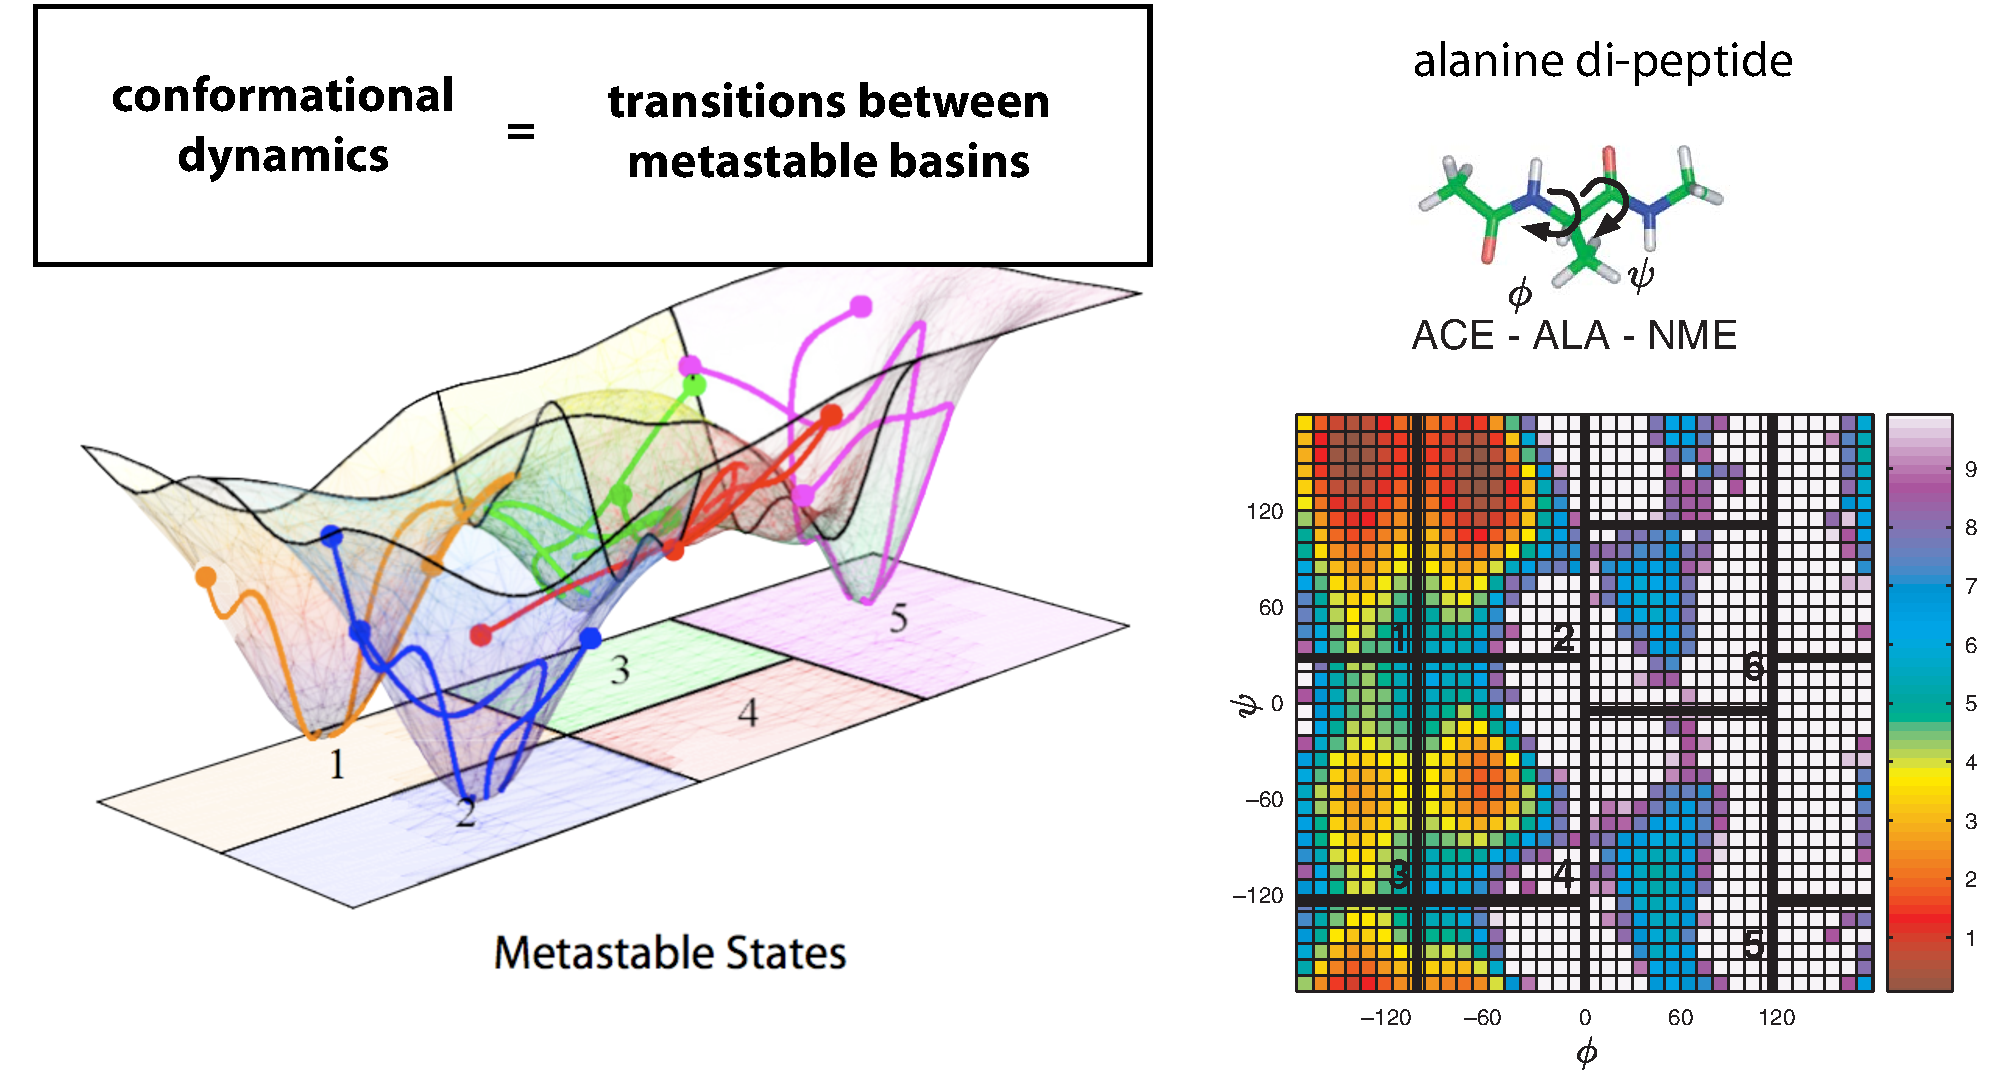
\includegraphics[width=1.0\textwidth]{MSMs}
%\caption{\label{fig:your-figure}Caption goes here.}
\end{figure}


\tiny
Huang, X., Bowman, G. R., Bacallado, S., \& Pande, V. S. (2009). PNAS, 106(47), 19765–19769.

Chodera, J. D., Swope, W. C., Pitera, J. W., \& Dill, K. A. (2006).  Multiscale Modeling \& Simulation, 5(4), 1214
\normalsize

\end{frame}


%%%%%%%%%%%%%%%%%%%%%%%%%%%%%%%
\begin{frame}{Advantages of Markov State Models}

We can obtain \textbf{long-timescale dynamics} from ensembled of textbf{short-timescale} trajectories 
\begin{figure}
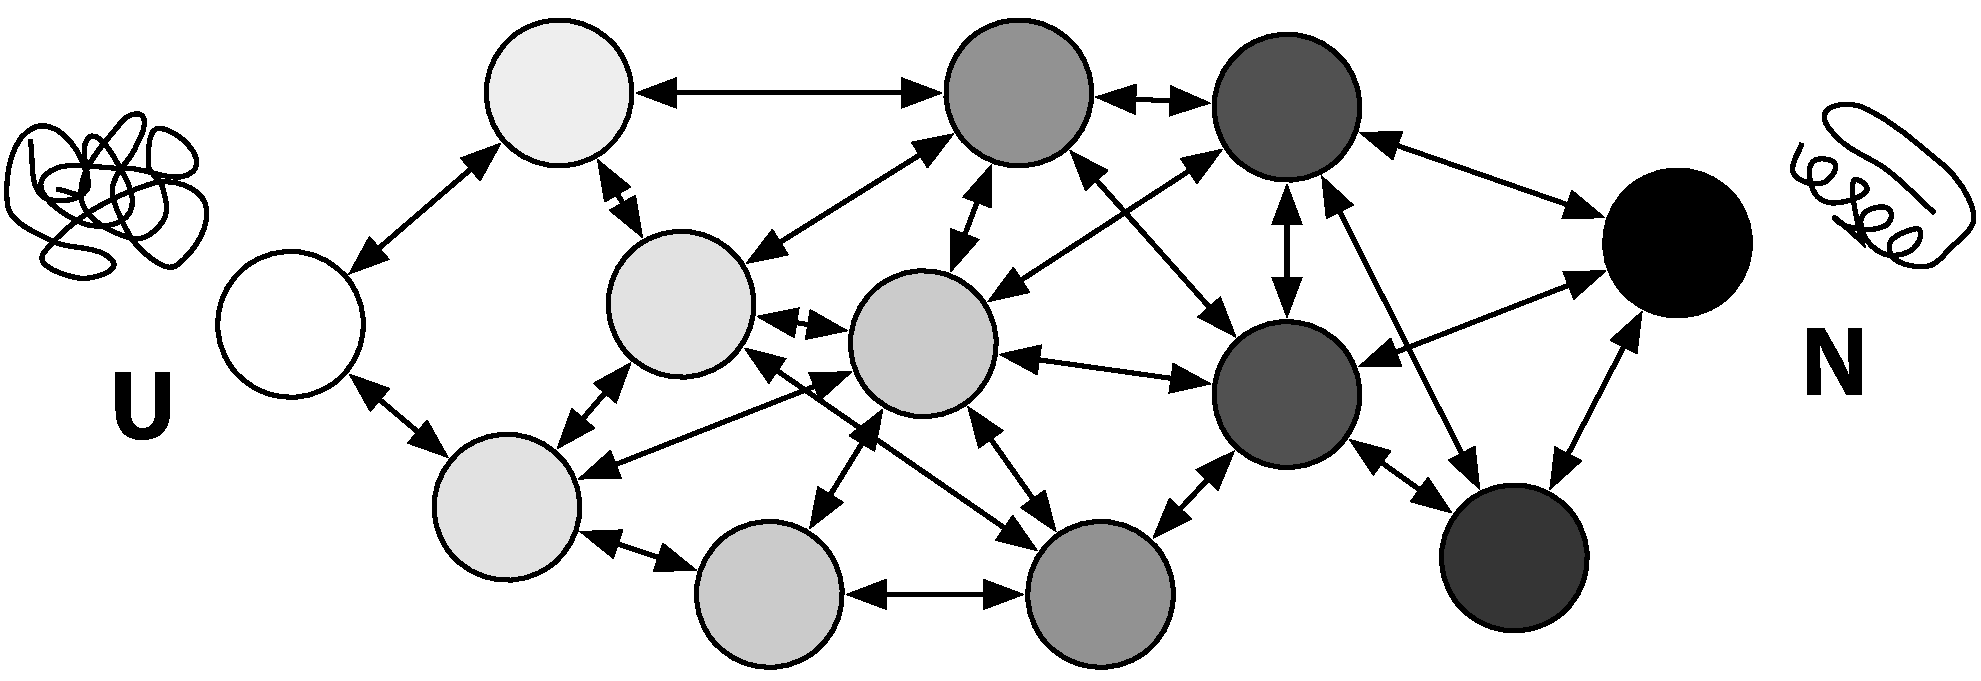
\includegraphics[width=1.0\textwidth]{network1}
%\caption{\label{fig:your-figure}Caption goes here.}
\end{figure}


\tiny
Chodera, Swope,  Pitera  and Dill. Multiscale Model. Simul. (2006), 5, 1214–1226

No\'{e} and Fischer Curr. Opin. Struct. Biol  (2008) 18(2): 154-162

Buchete and Hummer.  J. Phys. Chem. B 2008, 112, 6057-6069

No\'{e} F, Sch\"{u}tte C, Vanden-Eijnden E, Reich L, Weikl TR.  PNAS (2009) 106(45):19011-6.
\normalsize

\end{frame}

%%%%%%%%%%%%%%%%%%%%%%%%%%%%%%%
\begin{frame}{Advantages of Markov State Models}

We can use \textbf{adaptive sampling methods} to decrease our uncertainty in some quantity of interest (like the folding rate)  
\begin{figure}
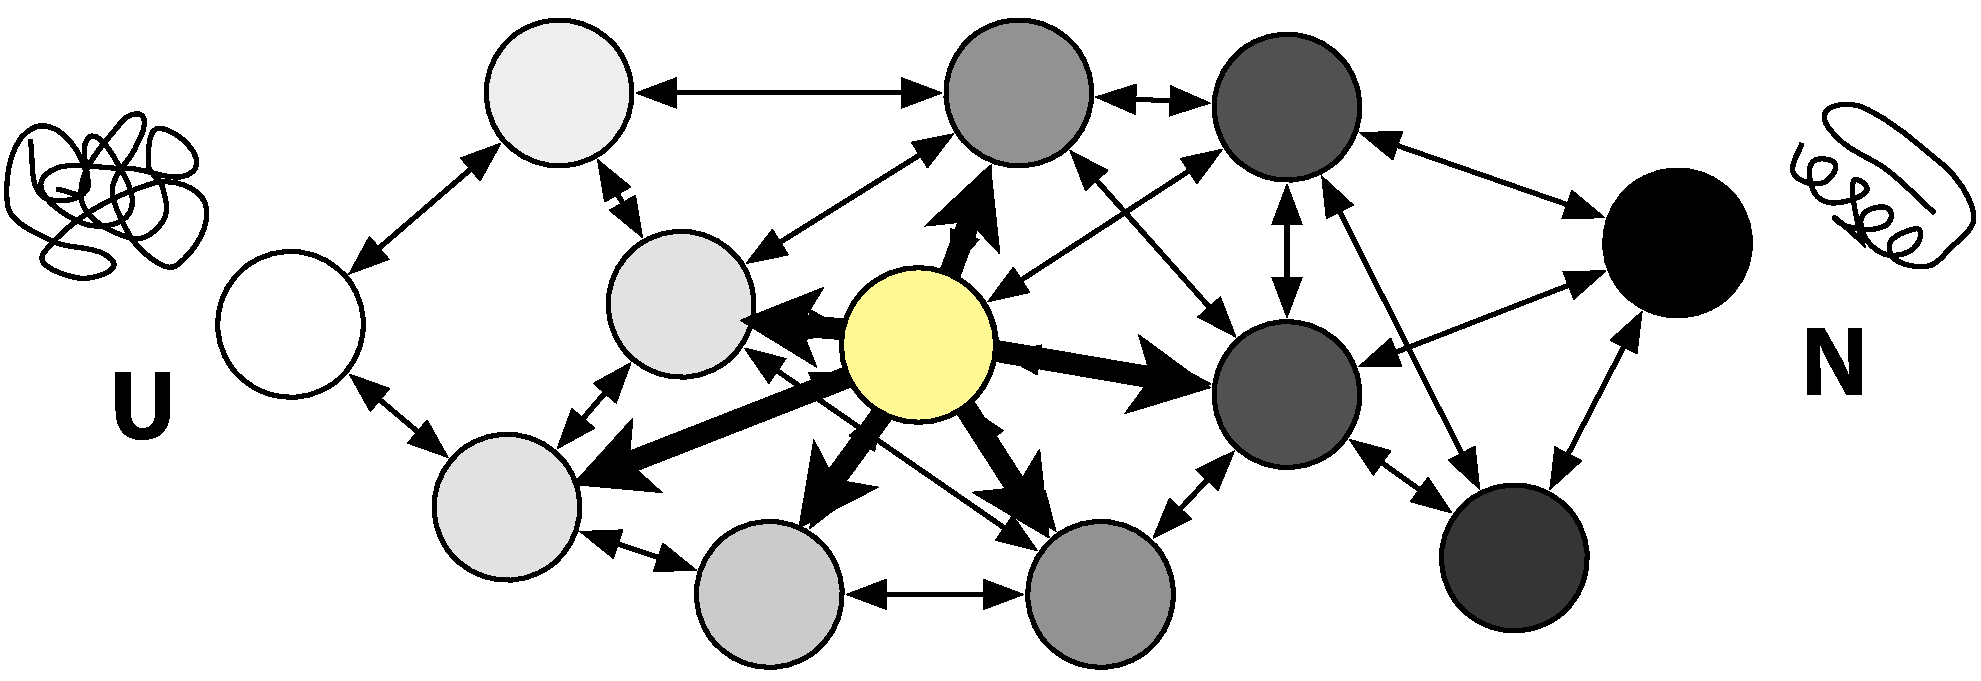
\includegraphics[width=1.0\textwidth]{network2}
%\caption{\label{fig:your-figure}Caption goes here.}
\end{figure}


\tiny
Singhal and Pande.  J. Chem. Phys. (2005) 123 204909

F. No\'{e}  J. Chem. Phys. (2008) 128, 244103

S. Bacallado, J. Chodera, and V. Pande.  J. Chem. Phys. (2009) 131, 045106. 

G. Bowman, D. Ensign and V. Pande , J. Chem. Theor. Comp. (2010) 6(3):  787–794

\normalsize

\end{frame}



%%%%%%%%%%%%%%%%%
\begin{frame}{Challenges in constructing Markov State Models}

\begin{itemize}
  \item What are the relevant metastable states?
  \item How do we validate the assumption that dynamics is ``Markovian''?
  \item How can estimate all the necessary rates?
  \item How can we make human sense of such huge networks?
\end{itemize}

\end{frame}

%%%%%%%%%%%%
\begin{frame}{The chemical master equation}

\begin{figure}
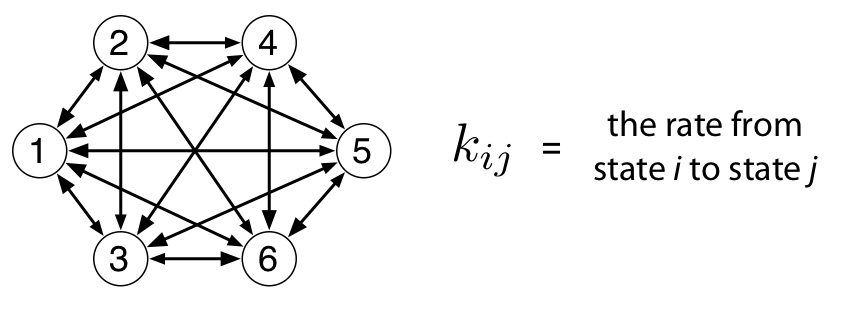
\includegraphics[width=0.6\textwidth]{n-state-kinetics}
%\caption{\label{fig:your-figure}Caption goes here.}
\end{figure}

There are $N$ states, whose populations change according to simple first-order kinetic rates
$$\frac{dp_1}{dt} = -(k_{12}+k_{13}+…+k_{1n})p_1 + k_{21} p_2 +k_{31} p_3 + ... +  k_{N1} p_n $$
$$\frac{dp_2}{dt} = k_{12} p_1 + -(k_{21}+k_{23}+…+k_{2N})p_2 + k_{32} p_3 + ... +  k_{N2} p_N $$
$$ ... $$
$$\frac{dp_N}{dt} = k_{1N} p_1 + k_{2N} p_2 + ...   -(k_{21}+k_{23}+…+k_{2N})p_2$$


\end{frame}


%%%%%%%%%%%%%%%%%%%%%%%%%%%%%%%
\begin{frame}{The chemical master equation}

This can be expressed succinctly as 
$$\frac{d}{dt} \mathbf{p} = \mathbf{K} \mathbf{p}$$
where $\mathbf{p}$(t) is the vector of state populations over time, and $\mathbf{K}$ is the rate matrix
$$\mathbf{K} =
 \begin{pmatrix}
  -\sum_{i \neq 1} k_{1i} & k_{21} & \cdots & k_{N1} \\
  k_{12} & -\sum_{i \neq 2}k_{2i} & \cdots & k_{N2} \\
  \vdots  & \vdots  & \ddots & \vdots  \\
  k_{1N} & k_{2N} & \cdots & -\sum_{i \neq N}k_{Ni}
 \end{pmatrix}
$$
*** Note that using this nomenclature, $K_{ji}$ is the rate of transition from state $i$ to state $j$

\end{frame}

\begin{frame}{Solving the master equation}

The most straightforward way to solve for $\mathbf{p}(t)$ is to transform coordinates to the eigenbasis of $\mathbf{K}$.  Let $\mathbf{V}$ be the matrix whose columns are (right) eigenvectors of $\mathbf{K}$. Then
$$\mathbf{K} \mathbf{V} = \mathbf{V} \mathbf{\Lambda} $$
where $\mathbf{\Lambda}$ is the diagonal matrix containing the eigenvalues of $\mathbf{K}$.  Let $\mathbf{p}'(t)$ be the populations in the new coordinate system, such that
$$\mathbf{V}\mathbf{p}' = \mathbf{p}$$
so that the master equation reads:

$$\frac{d}{dt} \mathbf{V}\mathbf{p}' = \mathbf{K} \mathbf{V}\mathbf{p}'$$

\end{frame}

\begin{frame}{Solving the master equation}

Applying $\mathbf{V}^{-1}$ yields
$$\mathbf{V}^{-1} \frac{d}{dt} \mathbf{V}\mathbf{p}' = \mathbf{V}^{-1} \mathbf{K} \mathbf{V}\mathbf{p}'$$
$$\frac{d}{dt} \mathbf{p}'=  \mathbf{\Lambda} \mathbf{p}'$$
We now have $N$ independent first-order equations whose solutions are
$$p_n'(t) = p_n'(0) \exp (\lambda_n t)$$
Transforming back to the original coordinate system, we get:
$$\mathbf{p}(t) = \sum_{i=1}^N \mathbf{v}_n [\mathbf{w}_n^T \mathbf{p}(0)] \exp (\lambda_n t)$$
where $\mathbf{v}_n$ and $\mathbf{w}_n$ are the right and left eigenvectors (respectively) of $\mathbf{K}$, whereby $p_n'(0) = (\mathbf{V}^{-1} \mathbf{p}(0))_n = (\mathbf{W}^T \mathbf{p}(0))_n$
\end{frame}


\begin{frame}{ME kinetics: a superposition of $N$ eigenmode relaxations}

The eigenvalues of $\mathbf{K}$ can be ordered $\lambda_1 > \lambda_2 > ... \lambda_N$, with $\lambda_1 = 0$ corresponding to the stationary state (i.e. equilibrium populations) $\mathbf{p}_{eq} = \mathbf{v}_1$, i.e.

$$\frac{d}{dt} \mathbf{p}_{eq} = \mathbf{K} \mathbf{p}_{eq}= 0$$
and the remaining eigenmodes $\mathbf{v}_n$ exponentially decaying with time constants $\tau_n = -1/\lambda_n$

\begin{figure}
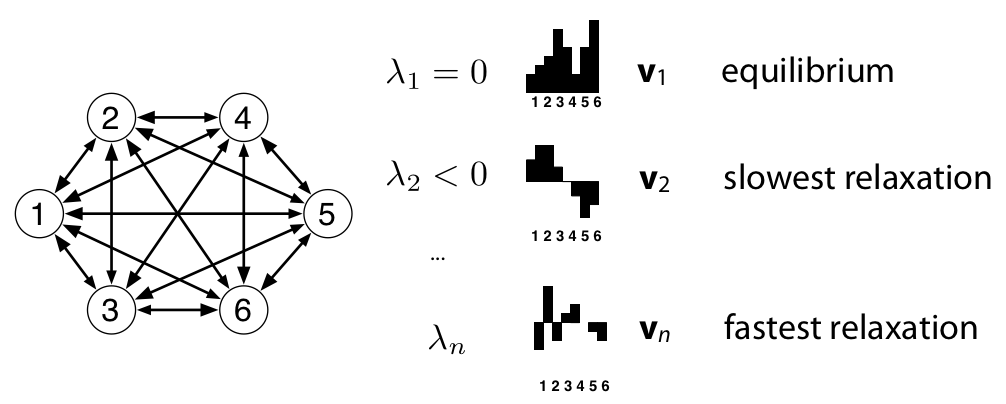
\includegraphics[width=0.8\textwidth]{eigenmodes}
%\caption{\label{fig:your-figure}Caption goes here.}
\end{figure}

\end{frame}



\begin{frame}{Protein Folding kinetics often appears two-state because there is a large gap in the spectrum of timescales}

\begin{figure}
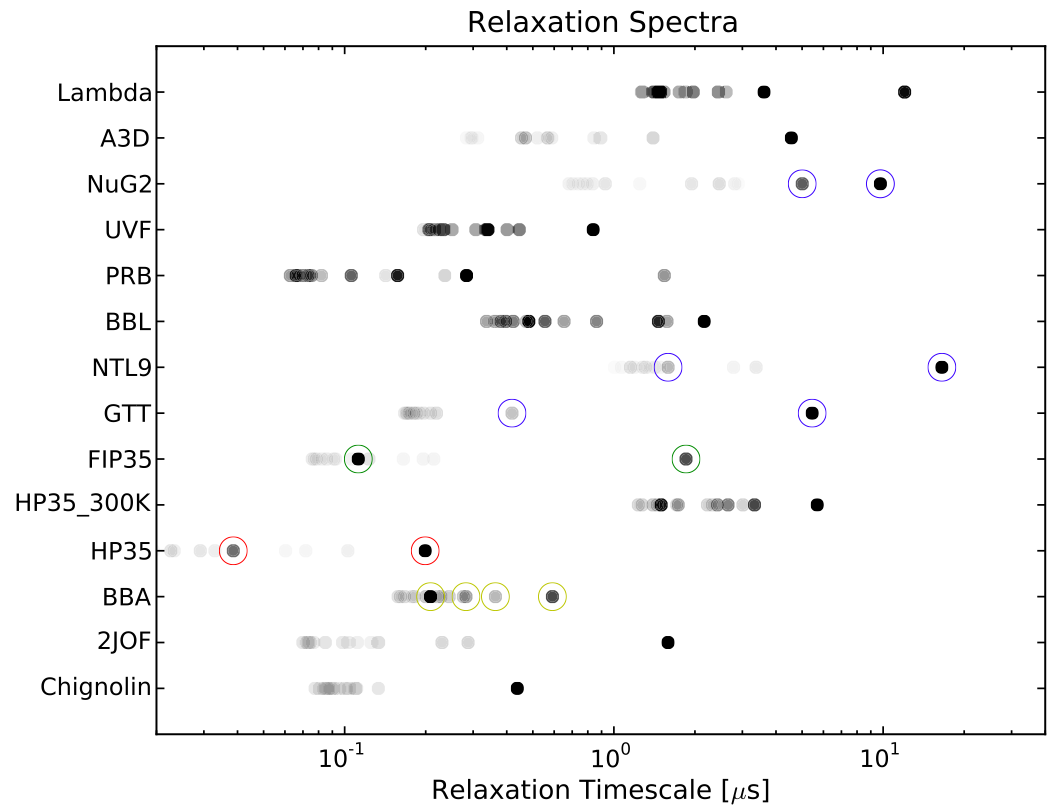
\includegraphics[width=0.8\textwidth]{beauchamp}
%\caption{\label{fig:your-figure}Caption goes here.}
\end{figure}

\tiny
Beauchamp, KA et al. (2012). Simple few-state models reveal hidden complexity in protein folding. PNAS doi:10.1073/pnas.1201810109
\normalsize

\end{frame}

\begin{frame}{Slowest eigenmodes for WW domain folding}

\begin{figure}
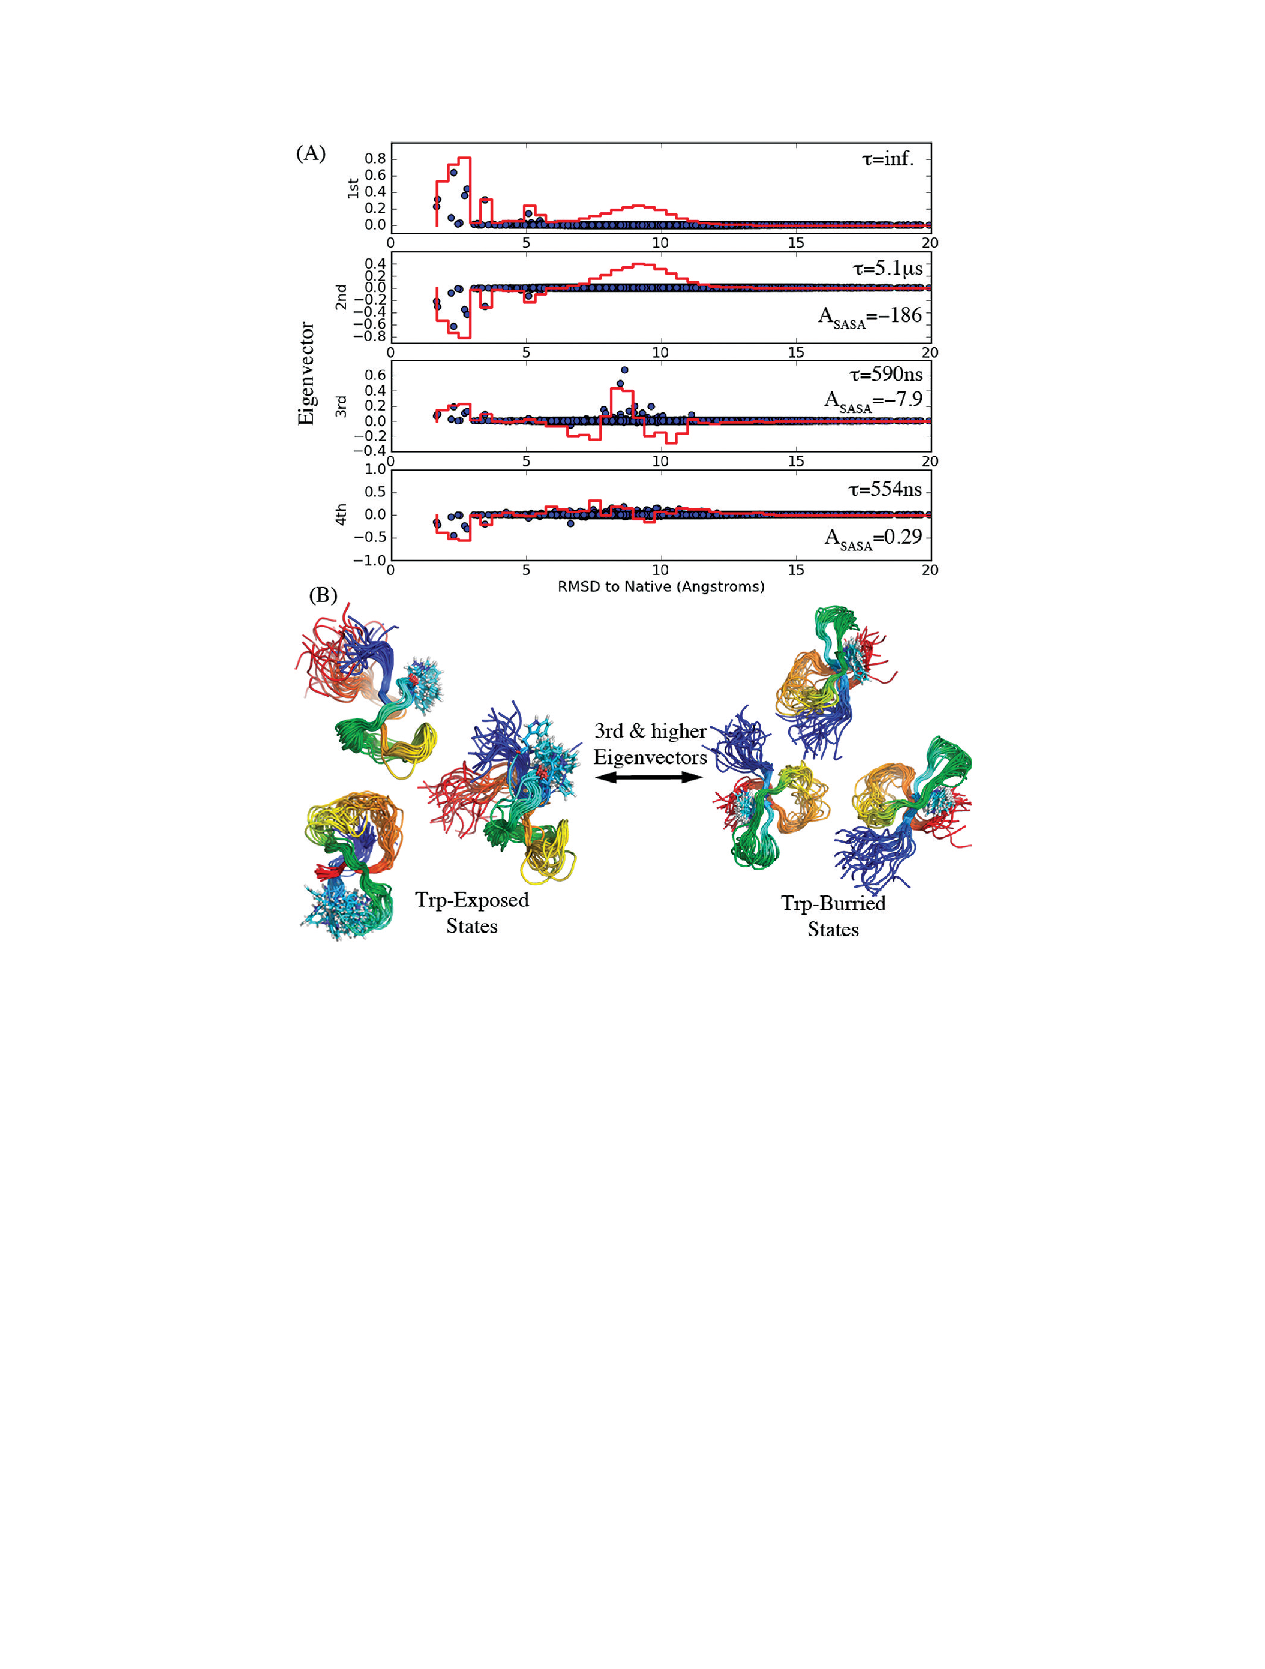
\includegraphics[width=0.6\textwidth]{ww-eigenmodes}
%\caption{\label{fig:your-figure}Caption goes here.}
\end{figure}

\tiny
Lane, TJ et al. (2011).  Markov state model reveals folding and functional dynamics in ultra-long MD trajectories. JACS, 133(45), 18413–18419. doi:10.1021/ja207470h
\normalsize

\end{frame}


\begin{frame}{Discrete-time Markov models}

\begin{figure}
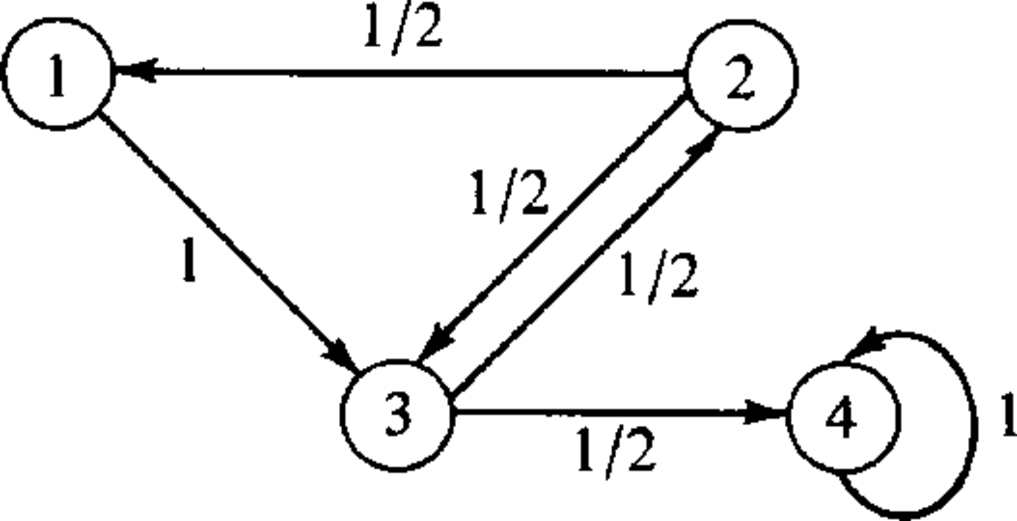
\includegraphics[width=0.4\textwidth]{markov}
%\caption{\label{fig:your-figure}Caption goes here.}
\end{figure}

A Markov Model describes population changes in discrete time intervals, using a \textit{transition matrix} $\mathbf{T}^{(\tau)}$, whose elements $T_{ji}$ are probability of transitioning from state $i$ to state $j$ in some time $\tau$.  The time evolution of $\mathbf{p}(t)$ can thus be obtained by iterated multiplcation:

$$\mathbf{p}(t+\tau) = \mathbf{T}^{(\tau)}\mathbf{p}(t)$$

From a practical standpoint, transition probabilities are more easily estimated from molecular simulations than rates.

\end{frame}



\begin{frame}{Discrete-time Markov models}

\begin{block}{Question}
What is the relationship between $\mathbf{T}^{(\tau)}$ and $\mathbf{K}$?
\end{block}

\vskip 1cm


Consider the time-evolution of populations according to the master equation $\frac{d}{dt}\mathbf{p}(t) = \mathbf{K} \mathbf{p}$. After some small time interval $\delta t << \tau$ has elapsed, the populations have changed by
$$\delta \mathbf{p} = \mathbf{K}\mathbf{p}(t) \delta t$$
so that 
$$\mathbf{p}(t+\delta t) = \mathbf{p}(t) + \delta \mathbf{p} = (\mathbf{1} + \mathbf{K} \delta t)\mathbf{p}(t)$$
\end{frame}


\begin{frame}{Discrete-time Markov models}

\begin{figure}
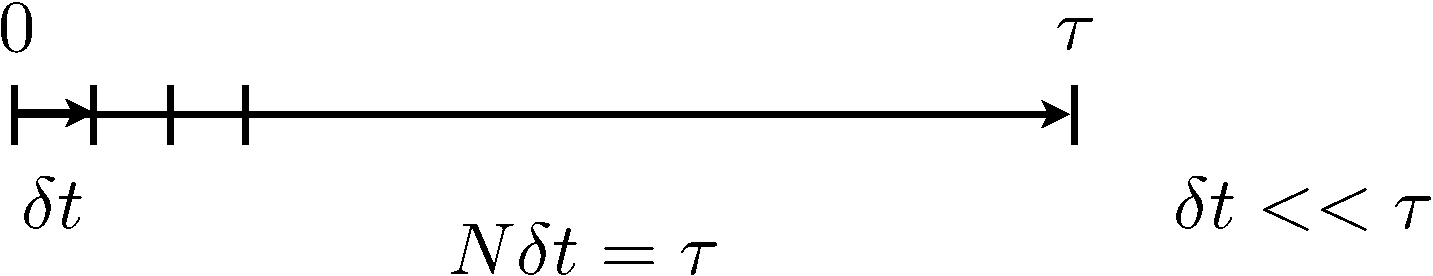
\includegraphics[width=0.8\textwidth]{tau-chopped}
%\caption{\label{fig:your-figure}Caption goes here.}
\end{figure}

If the time window $\tau$ is divided up into $N$  small intervals (such that $N \delta t = \tau$), iteration of the above  yields

$$\mathbf{p}(t+N\delta t) = (\mathbf{1} + \mathbf{K} \delta t)^N\mathbf{p}(t)$$

Taking the limit where $N \rightarrow \infty$ and $\delta t \rightarrow 0$, we get

$$\mathbf{p}(t+\tau) = \lim_{N \rightarrow \infty} (\mathbf{1} + \mathbf{K} \frac{\tau}{N})^N\mathbf{p}(t) = \exp(\mathbf{K}\tau)\mathbf{p}(t)$$

Therefore,
$$\mathbf{T}^{(\tau)} = \exp(\mathbf{K}\tau)$$

\end{frame}


\begin{frame}{$\mathbf{T}^{(\tau)}$ and $\mathbf{K}$ share eigenvectors }

If we write the matrix exponential as an Euler series, we can easily see that $\mathbf{T}^{(\tau)}$ and $\mathbf{K}$ share eigenvectors.  

$$\mathbf{T}^{(\tau)}\mathbf{v}_n = \exp(\mathbf{K}\tau) \mathbf{v}_n$$
$$= [1 + \mathbf{K}\tau + \frac{1}{2!}\mathbf{K}^2\tau^2 + \frac{1}{3!}\mathbf{K}^3\tau^3 + ...]  \mathbf{v}_n$$
$$= [1 + \lambda_n\tau + \frac{1}{2!}\lambda_n^2\tau^2 + \frac{1}{3!}\lambda_n^3\tau^3 + ...]  \mathbf{v}_n$$
$$ \mathbf{T}^{(\tau)}\mathbf{v}_n = \exp(\lambda_n \tau) \mathbf{v}_n$$
The eigenvalues of $ \mathbf{T}^{(\tau)}$, $\mu_n$, are related to $\lambda_n$ by
$$ \lambda_n = \log(\mu_n)/\tau$$
i.e. \textbf{implied timescales} $\boxed{ \tau_n = \frac{\tau}{-\log(\mu_n)}  }$
\end{frame}


%%%%%%%%%%%%%%%%%%%%%%%%%%%%%%%%%%%%%%%%
\begin{frame}{Constructing Markov State Models (MSMs)}

\begin{itemize}
  \item Identify metastable microstates
  \item Estimate $\mathbf{T}^{(\tau)}$ from observed transition counts
  \item Validation:
  \begin{itemize}
      \item Is our choice of $\tau$ suitable?
      \item Does the Markov property hold?
      \item Does the model recapitulate the raw simulation data?
  \end{itemize}
  \item $\mathbf{T}^{(\tau)}$ provides a complete description of ME kinetics
\end{itemize}


\end{frame}

%%%%%%%%%%%%%%%%%%%%%%%%%%%%%%%%%%%%%%%%
\begin{frame}{MSMBuilder}

\begin{figure}
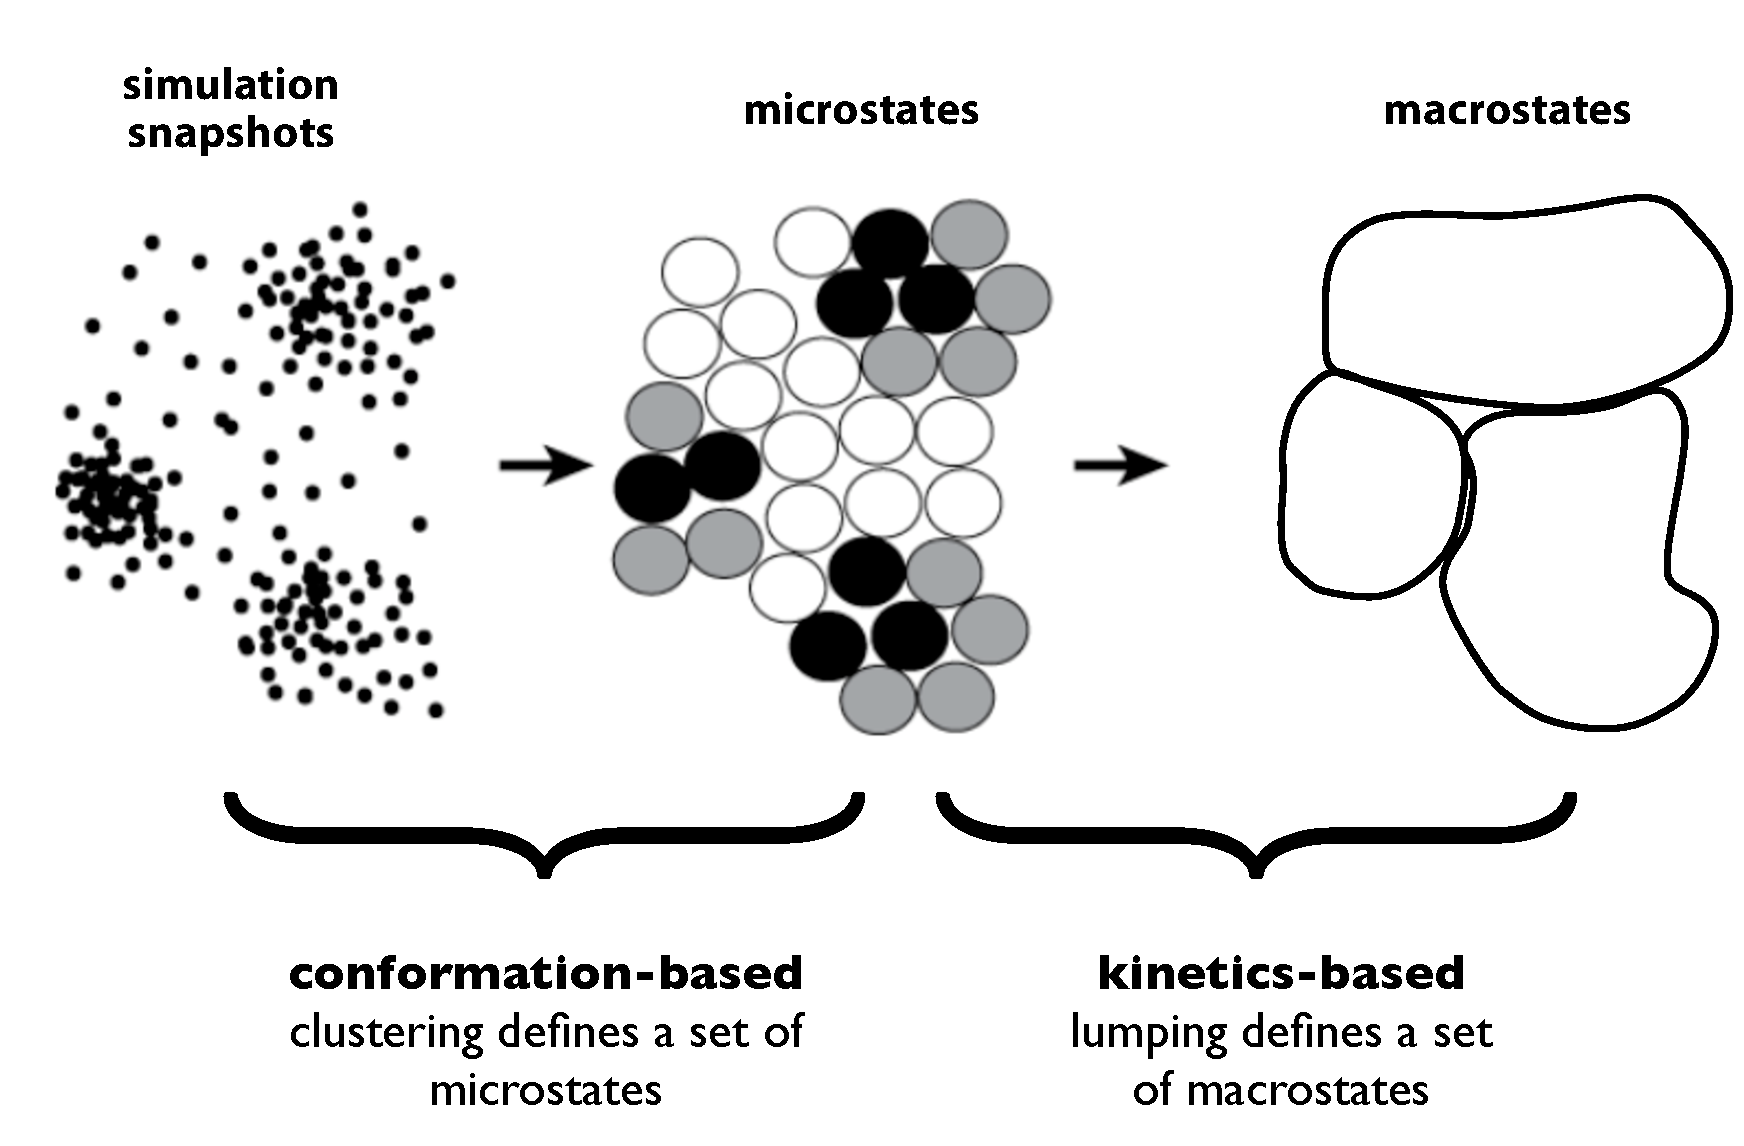
\includegraphics[width=1.0\textwidth]{msmbuilder}
%\caption{\label{fig:your-figure}Caption goes here.}
\end{figure}

\tiny
Beauchamp, K. A., Bowman, G. R., Lane, T. J., Maibaum, L., Haque, I. S. and Pande, V. S. (2011). MSMBuilder2: Modeling Conformational Dynamics on the Picosecond to Millisecond Scale. JCTC, 7(10), 3412–3419. doi:10.1021/ct200463m
Pande, V. S., Beauchamp, K., and  Bowman, G. R. (2010). Everything you wanted to know about Markov State Models but were afraid to ask. Methods, 52(1), 99–105. doi:10.1016/j.ymeth.2010.06.002
\normalsize
\end{frame}

%%%%%%%%%%%%%%%%%%%%%%%%%%%%%%%%%%%%%%%%
\begin{frame}{MSMBuilder is on github}

\begin{figure}
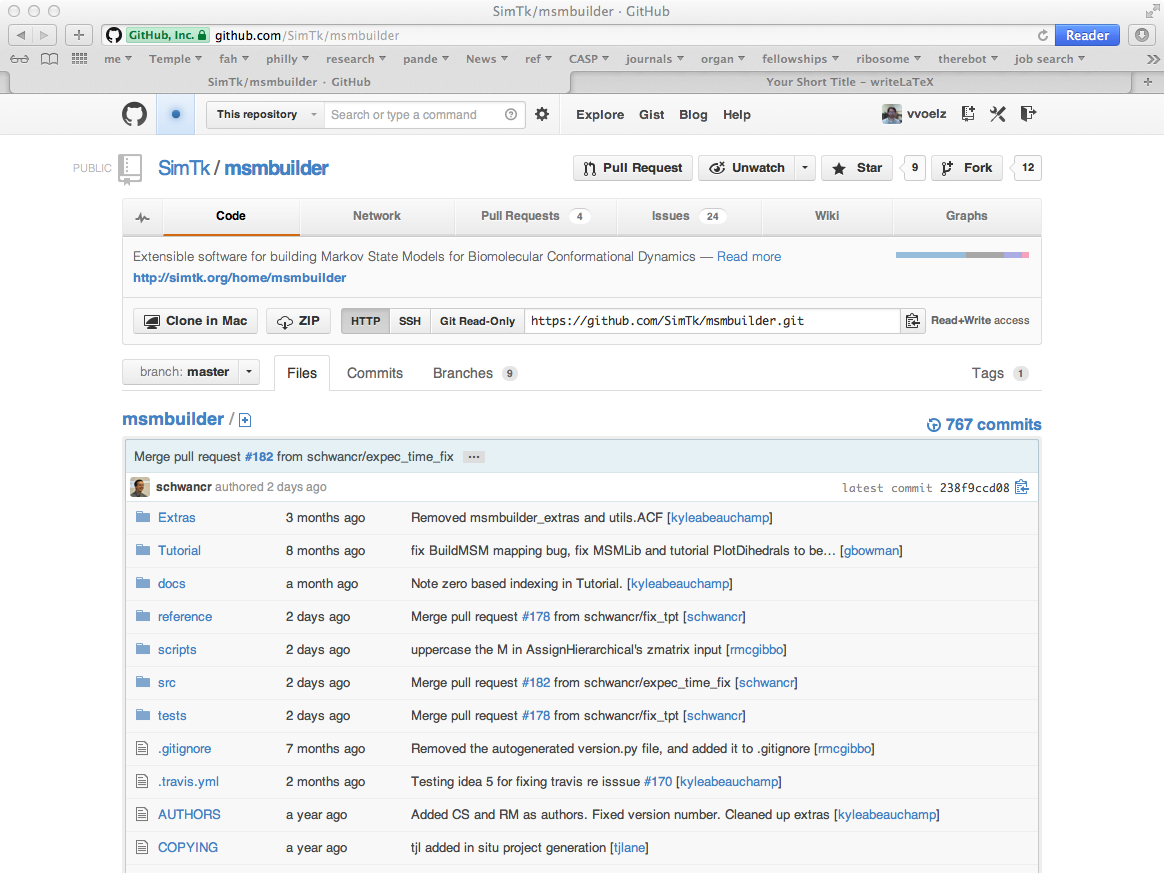
\includegraphics[width=1.0\textwidth]{github}
%\caption{\label{fig:your-figure}Caption goes here.}
\end{figure}

\end{frame}



%%%%%%%%%%%%%%%%%%%%%%%%%%%%%%%%%%%%%%%%
\begin{frame}{Conformational Clustering }

On short timescales, geometric distance is a good proxy for kinetic distance.

\begin{itemize}
  \item $k$-centers and hybrid $k$-centers/$k$-medoid clustering
  \item hierachical clustering (Ward's algorithm) - takes a LOT of memory
  \item Many distance metrics available in MSMBuilder
  \begin{itemize}
      \item rmsd
      \item dihedral
      \item contact maps 
      \item user-defined (extensible code)
  \end{itemize}
  \item tICA method for projecting onto the degrees of freedom with the slowest correlated motions (Schwantes et al 2013, Perez-Hernandez et al 2013)
\end{itemize}

\tiny
Perez-Hernandez, G., Paul, F., Giorgino, T., De Fabritiis, G., and Noé, F. (2013). Identification of slow molecular order parameters for Markov model construction. arXiv preprint arXiv:1302.6614.

Schwantes, C. R. and Pande, V. S. (2013). Improvements in Markov State Model Construction Reveal Many Non-Native Interactions in the Folding of NTL9. Journal of Chemical Theory and Computation, 9(4), 2000–2009. doi:10.1021/ct300878a


\end{frame}

%%%%%%%%%%%%%%%%%%%%%%%%%%%%%%%%%%%%%%%%
\begin{frame}{How many microstates do we need?}
\begin{itemize}
    \item Too few microstates will fail to capture the correct separation of timescales
    \item Too many microstates will suffer from poor statistical sampling 
\end{itemize}
\begin{figure}
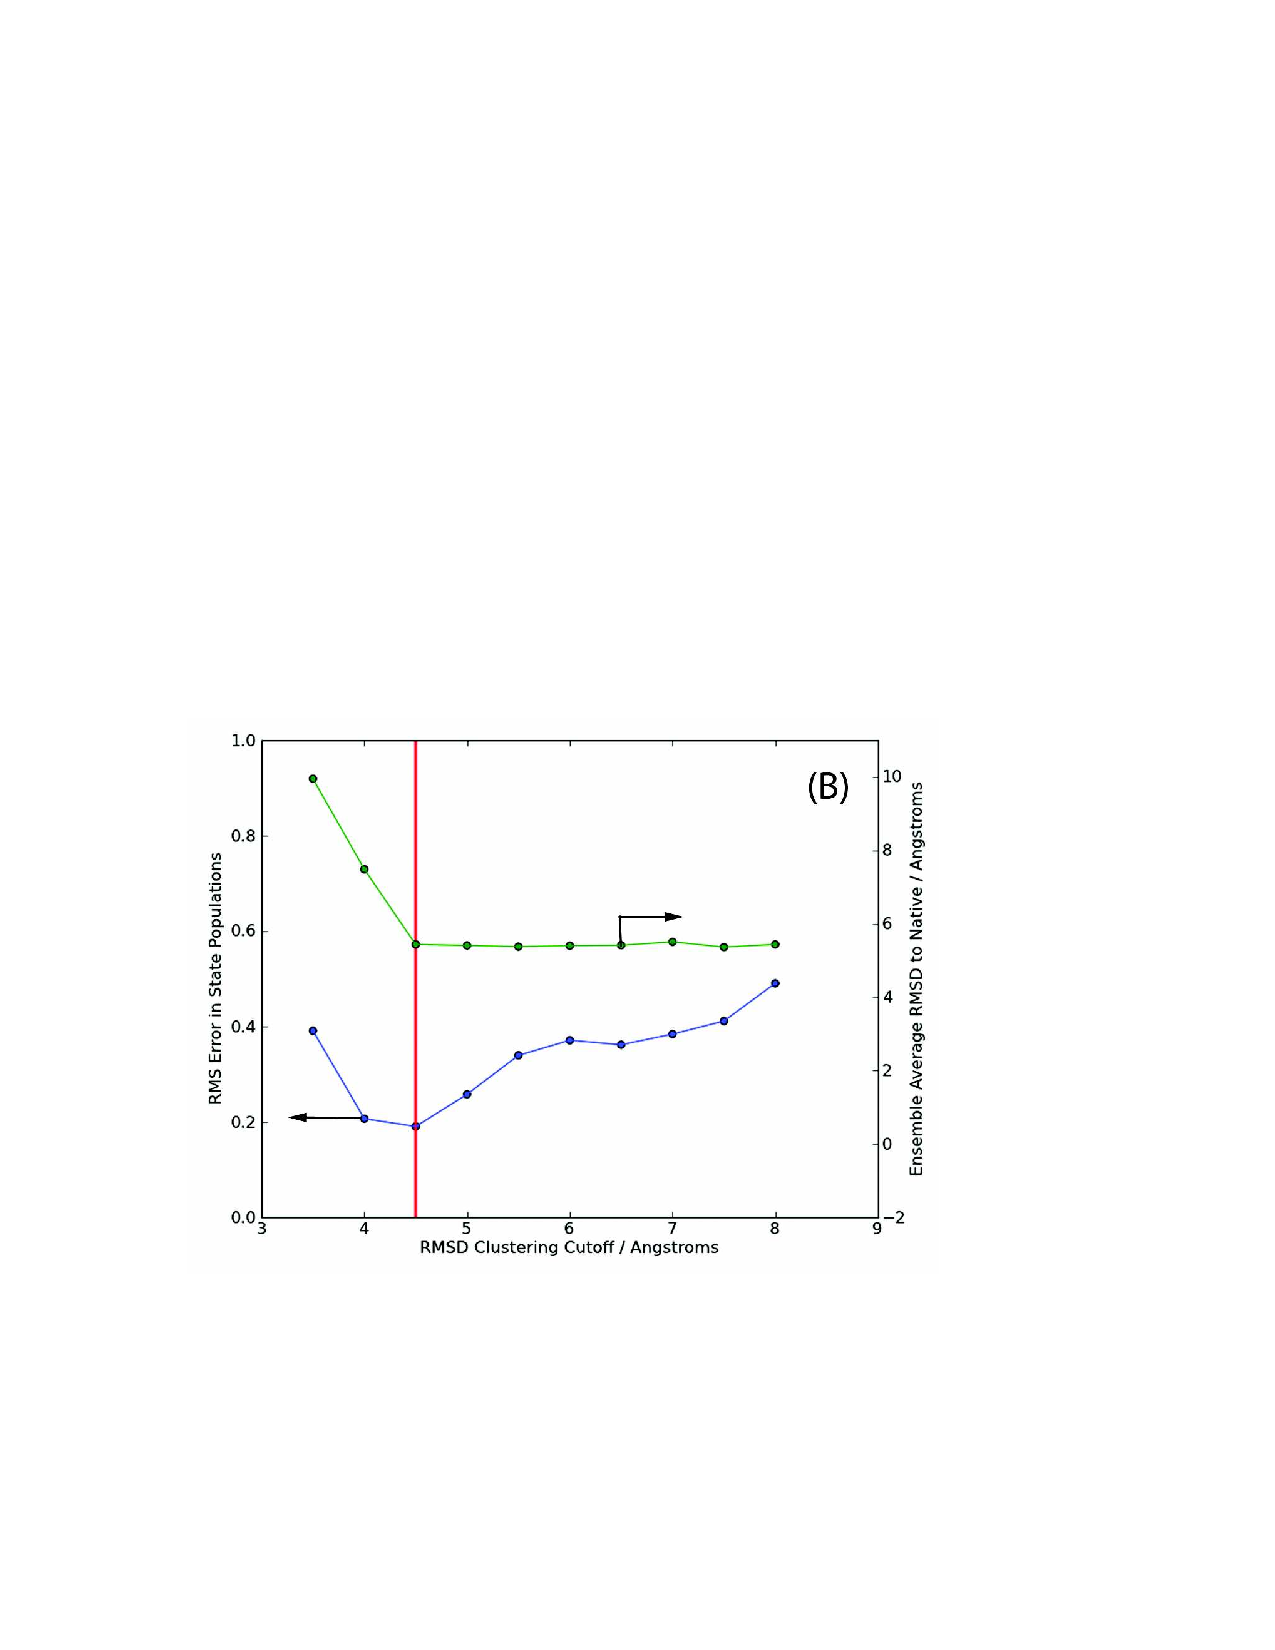
\includegraphics[width=0.65\textwidth]{ww-clustering}
%\caption{\label{fig:your-figure}Caption goes here.}
\end{figure}

\tiny
Lane, TJ et al. (2011).  Markov state model reveals folding and functional dynamics in ultra-long MD trajectories. JACS, 133(45), 18413–18419. doi:10.1021/ja207470h
\normalsize

\end{frame}



%%%%%%%%%%%%%%%%%%%%%%%%%%%%%%%%%%%%%%%%
\begin{frame}{Estimating $\mathbf{T}^{(\tau)}$ that obeys detailed balance}

In practice, we observe a finite set of (non-equilibrium) counts $\mathbf{C}^{(\tau)}$.  Simply (column-)normalizing $\mathbf{C}$ will \textit{not} produce a transition matrix that obeys detailed balance

$$ T_{ji} (\mathbf{p}_{eq})_i = T_{ij} (\mathbf{p}_{eq})_j    $$

Many methods exist to estimate $\mathbf{T}$

\begin{itemize}
    \item Symmetrization: $\mathbf{C}' = (\mathbf{C} + \mathbf{C}^T)/2$
    \item MLE: Find $\mathbf{T}$ that maximizes $P(\mathbf{C}|\mathbf{T})$ subject to a detailed balance constraint and/or Bayesian prior $P(\mathbf{C})$
    \item Edge-reinforced walk estimators (Bacallado et al.)
\end{itemize}


\tiny
Beauchamp, K. A., Bowman, G. R., Lane, T. J., Maibaum, L., Haque, I. S. and Pande, V. S. (2011). MSMBuilder2: Modeling Conformational Dynamics on the Picosecond to Millisecond Scale. JCTC, 7(10), 3412–3419. doi:10.1021/ct200463m
Prinz, J.-H., Wu, H., Sarich, M., Keller, B., Senne, M., Held, M., et al. (2011). Markov models of molecular kinetics: generation and validation. The Journal of Chemical Physics, 134(17), 174105. doi:10.1063/1.3565032
Bacallado, S., Chodera, J. D., \& Pande, V. (2009). Bayesian comparison of Markov models of molecular dynamics with detailed balance constraint. The Journal of Chemical Physics, 131(4), 045106. doi:10.1063/1.3192309

\end{frame}


%%%%%%%%%%%%%%%%%%%%%%%%%%%%%%%%%%%%%%%%
\begin{frame}{Choosing a lagtime}
\begin{itemize}
    \item Construct $\mathbf{T}^{(\tau)}$ for many different $\tau$ and compute the implied timescales $\tau_n$.
    \item Good models should have a``plateau'' region where the $\tau_n$ are relatively insensitive to lag time.
    \item No\'e et al. have shown that discretization errors can only serve to \textit{underestimate} timescales
\end{itemize}
\begin{figure}
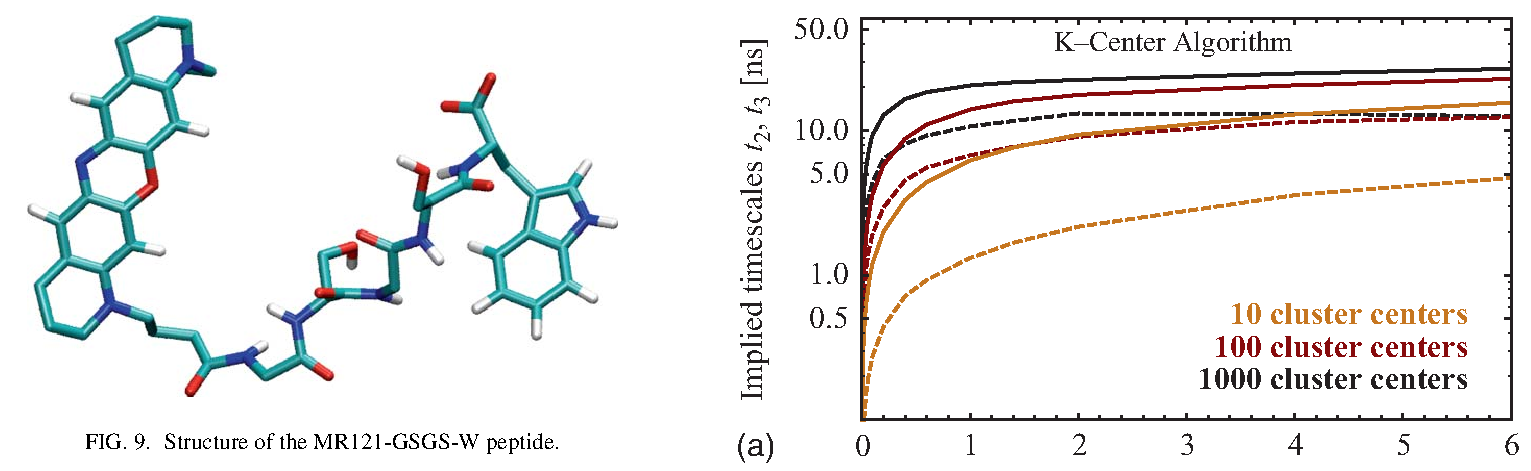
\includegraphics[width=0.9\textwidth]{MR121-GSGS-W}
%\caption{\label{fig:your-figure}Caption goes here.}
\end{figure}

\tiny
 Prinz, J.-H., Wu, H., Sarich, M., Keller, B., Senne, M., Held, M., Chodera, J. D., et al. (2011). The Journal of Chemical Physics, 134(17), 174105.
\normalsize

\end{frame}



%%%%%%%%%%%%%%%%%%%%%%%%%%%%%%%%%%%%%%%%
\begin{frame}{Choosing the best lagtime}

\begin{figure}
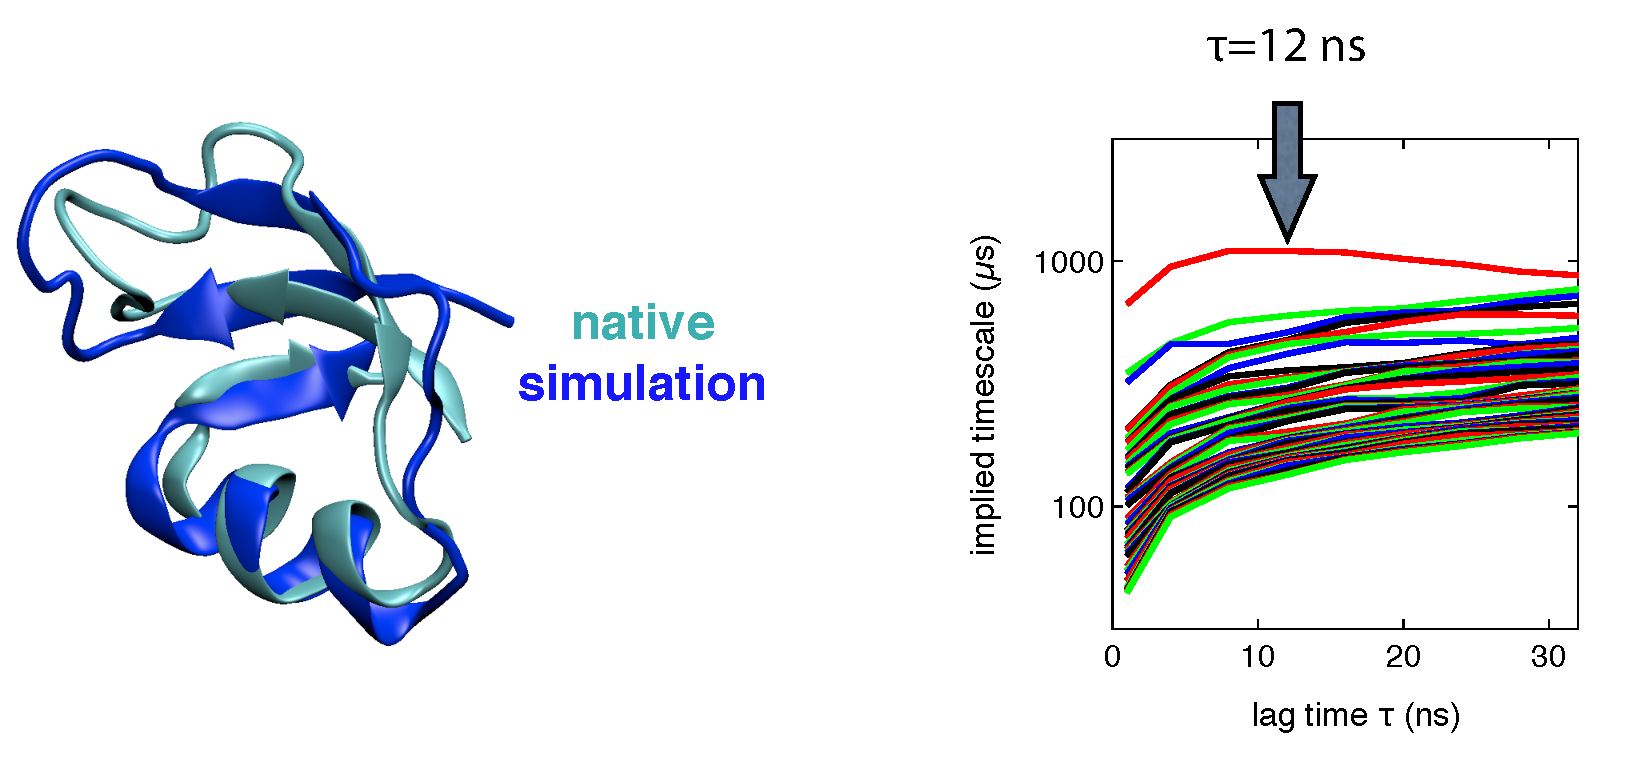
\includegraphics[width=0.9\textwidth]{ntl9-lagtimes}
%\caption{\label{fig:your-figure}Caption goes here.}
\end{figure}

\begin{itemize}
    \item NTL9(1-39) has a folding time of \~1 ms
    \item 1.52 ms of simulation data (1.5 million 1-ns snapshots) were clustered ($k$-centers) into 100,000 microstates. 
    \item The microstates had an average radius of \~4.5 \AA
    \item Timescale gap indicates apparent two-state folding
    \item Slowest timescale (\~1 ms) is close to experimental folding time
\end{itemize}

\tiny
Voelz VA, Bowman GR, Beauchamp KA and Pande VS. JACS (2010) 132 (5), 1526-1528.
\normalsize

\end{frame}

%%%%%%%%%%%%%%%%%%%%%%%%%%%%%%%%%%%%%%%%
\begin{frame}{Validation of MSMs: The Chapman-Kolmogorov test}

A strong test of the Markov property is the Chapman-Kolmogorov test, which states that

$$[\mathbf{T}^{(\tau)} ]^k \approx \mathbf{T}^{(k \tau)} $$

In practice, a test of this condition is performed by propagating some initial distribution of population $\mathbf{p}(0)$ (often set to $\delta_i$ for some state(s) of interest $i$)


\begin{figure}
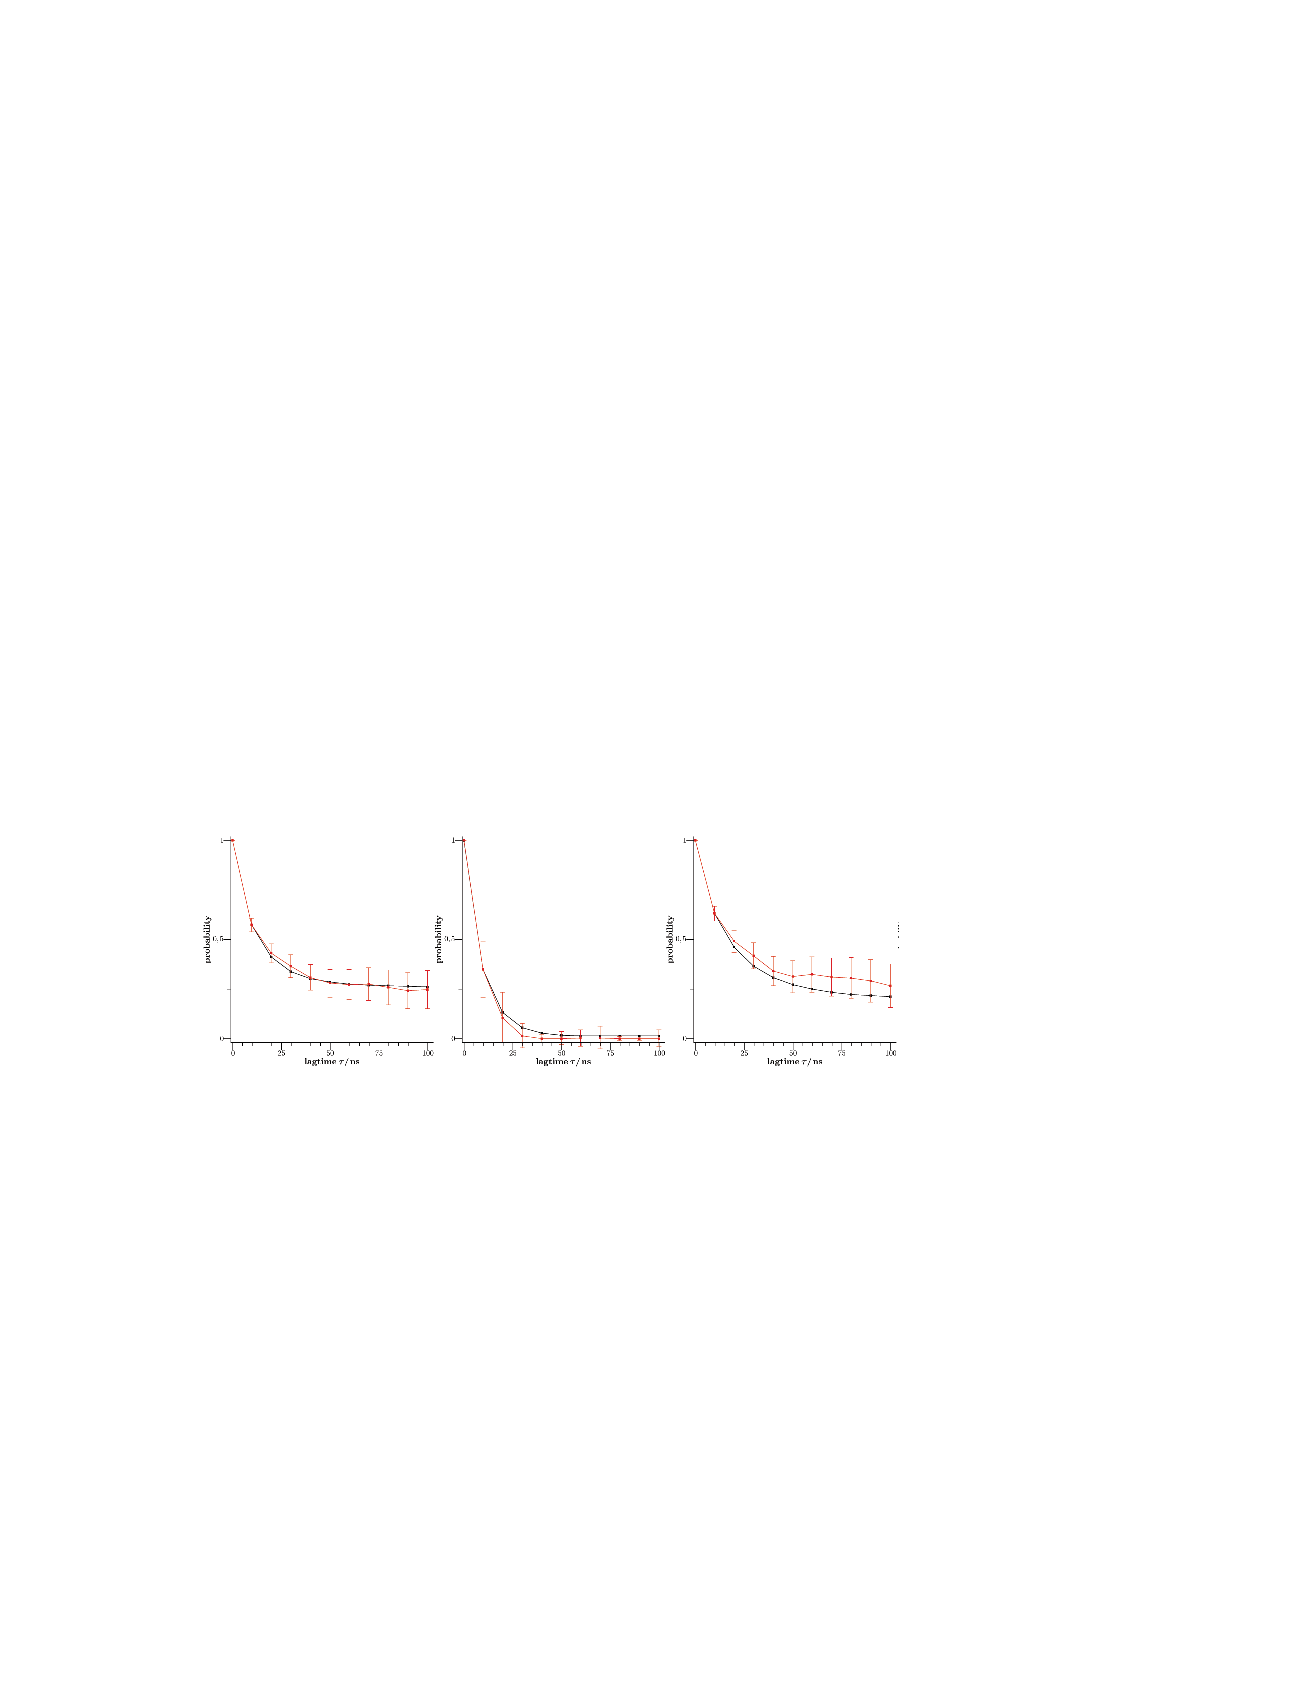
\includegraphics[width=0.8\textwidth]{CK-MR121}
%\caption{\label{fig:your-figure}Caption goes here.}
\end{figure}


\tiny
Senne, M., Trendelkamp-Schroer, B., Mey, A. S. J. S., Sch\"{u}tte, C., \& No\'{e}, F. (2012). EMMA: A Software Package for Markov Model Building and Analysis. Journal of Chemical Theory and Computation, 8(7), 2223–2238. doi:10.1021/ct300274u
\normalsize

\end{frame}


%%%%%%%%%%%%%%%%%%%%%%%%%%%%%%%%%%%%%%%%
\begin{frame}{Validation of MSMs: Autocorrelation Functions}

Another strong test of MSM validity is to compare autocorrelation functions for some order parameter or experimental observable

\begin{figure}
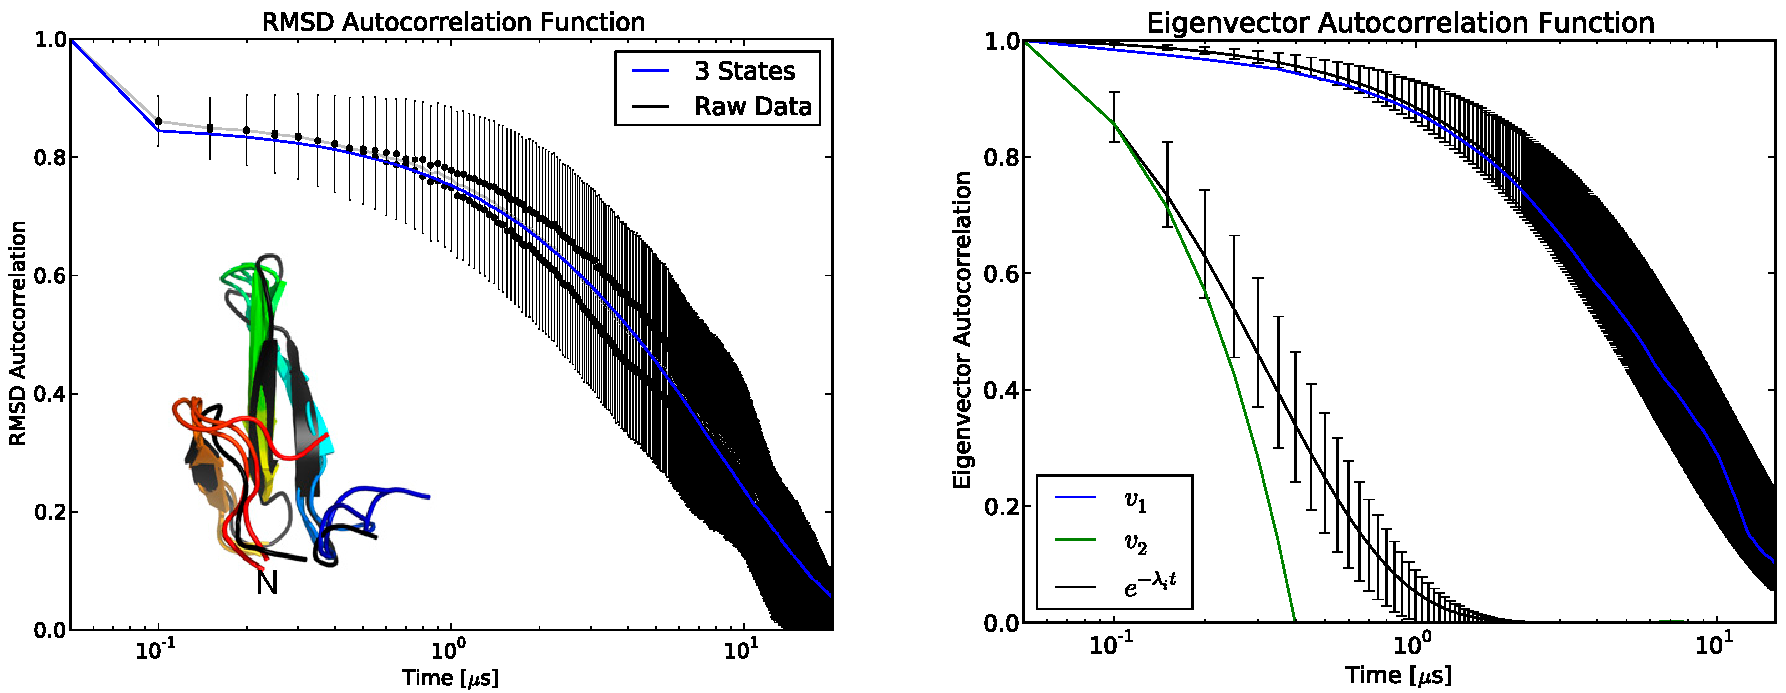
\includegraphics[width=1.0\textwidth]{GTT-autocorrelation}
%\caption{\label{fig:your-figure}Caption goes here.}
\end{figure}

\tiny
Beauchamp, KA et al. (2012). Simple few-state models reveal hidden complexity in protein folding. PNAS doi:10.1073/pnas.1201810109
\normalsize

\end{frame}


%%%%%%%%%%%%%%%%%%%%%%%%%%%%%%%%%%%%%%%%
\begin{frame}{The big picture:  MSMs are doing a good job reproducing experimental folding timescales}


\begin{figure}
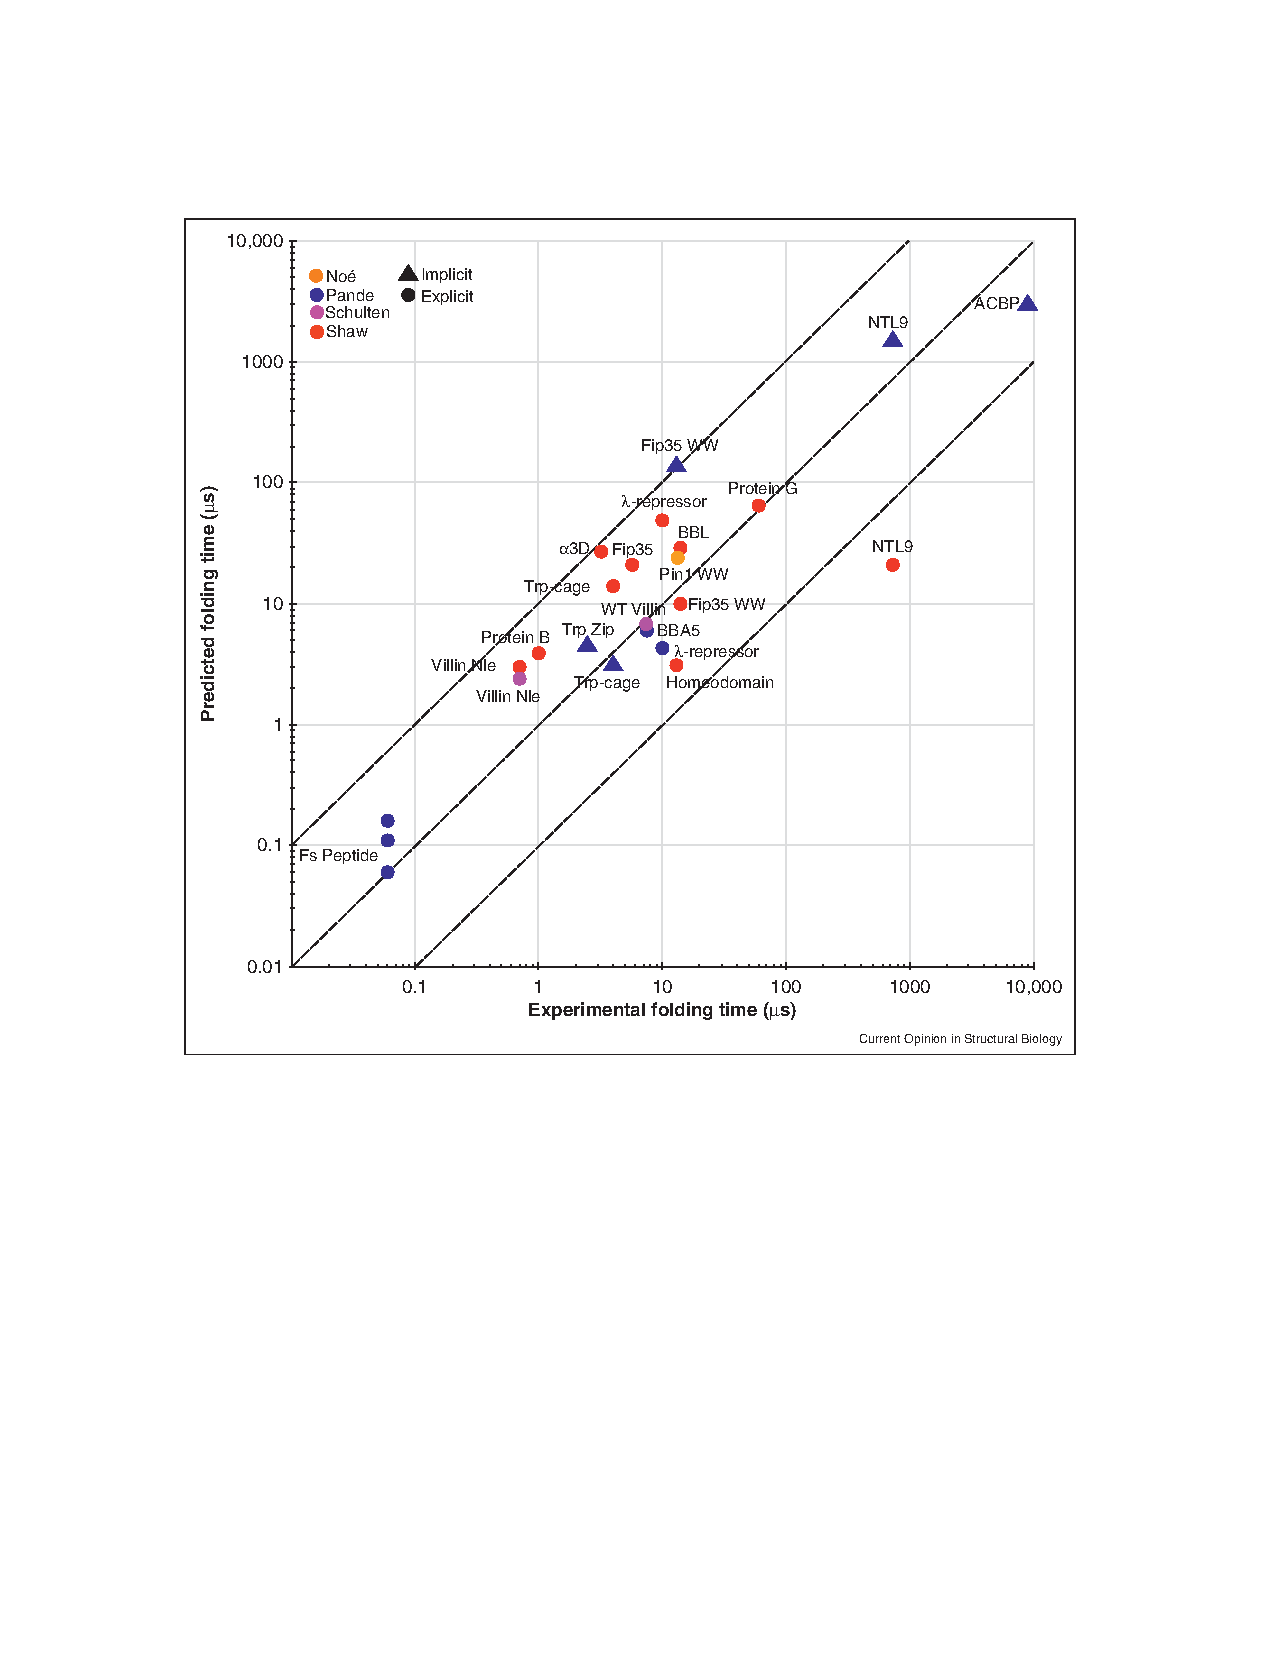
\includegraphics[width=0.65\textwidth]{MSM-scatter}
%\caption{\label{fig:your-figure}Caption goes here.}
\end{figure}

\tiny
Lane, T. J., Shukla, D., Beauchamp, K. A., \& Pande, V. S. (2012). To milliseconds and beyond: challenges in the simulation of protein folding. Current opinion in structural biology, 1–8. doi:10.1016/j.sbi.2012.11.002
\normalsize

\end{frame}


%%%%%%%%%%%%%%%%%%%%%%%%%%%%%%%%%%
\begin{frame}{Coarse-graining an MSM into macrostates makes it "human readable"}

\begin{block}{Question}
How can we make sense all the microscopic detail in kinetic network models?
\end{block}

\begin{itemize}
  \item Kinetics-based \textit{lumping} into macrostates
  \item Transition Path Theory (TPT)
\end{itemize}

\vskip 1cm

\end{frame}


%%%%%%%%%%%%%%%%%%%%%%%%%%%%%%%%%%
\begin{frame}{Automated algorithms for lumping microstates into macrostates by metastability}


\begin{figure}
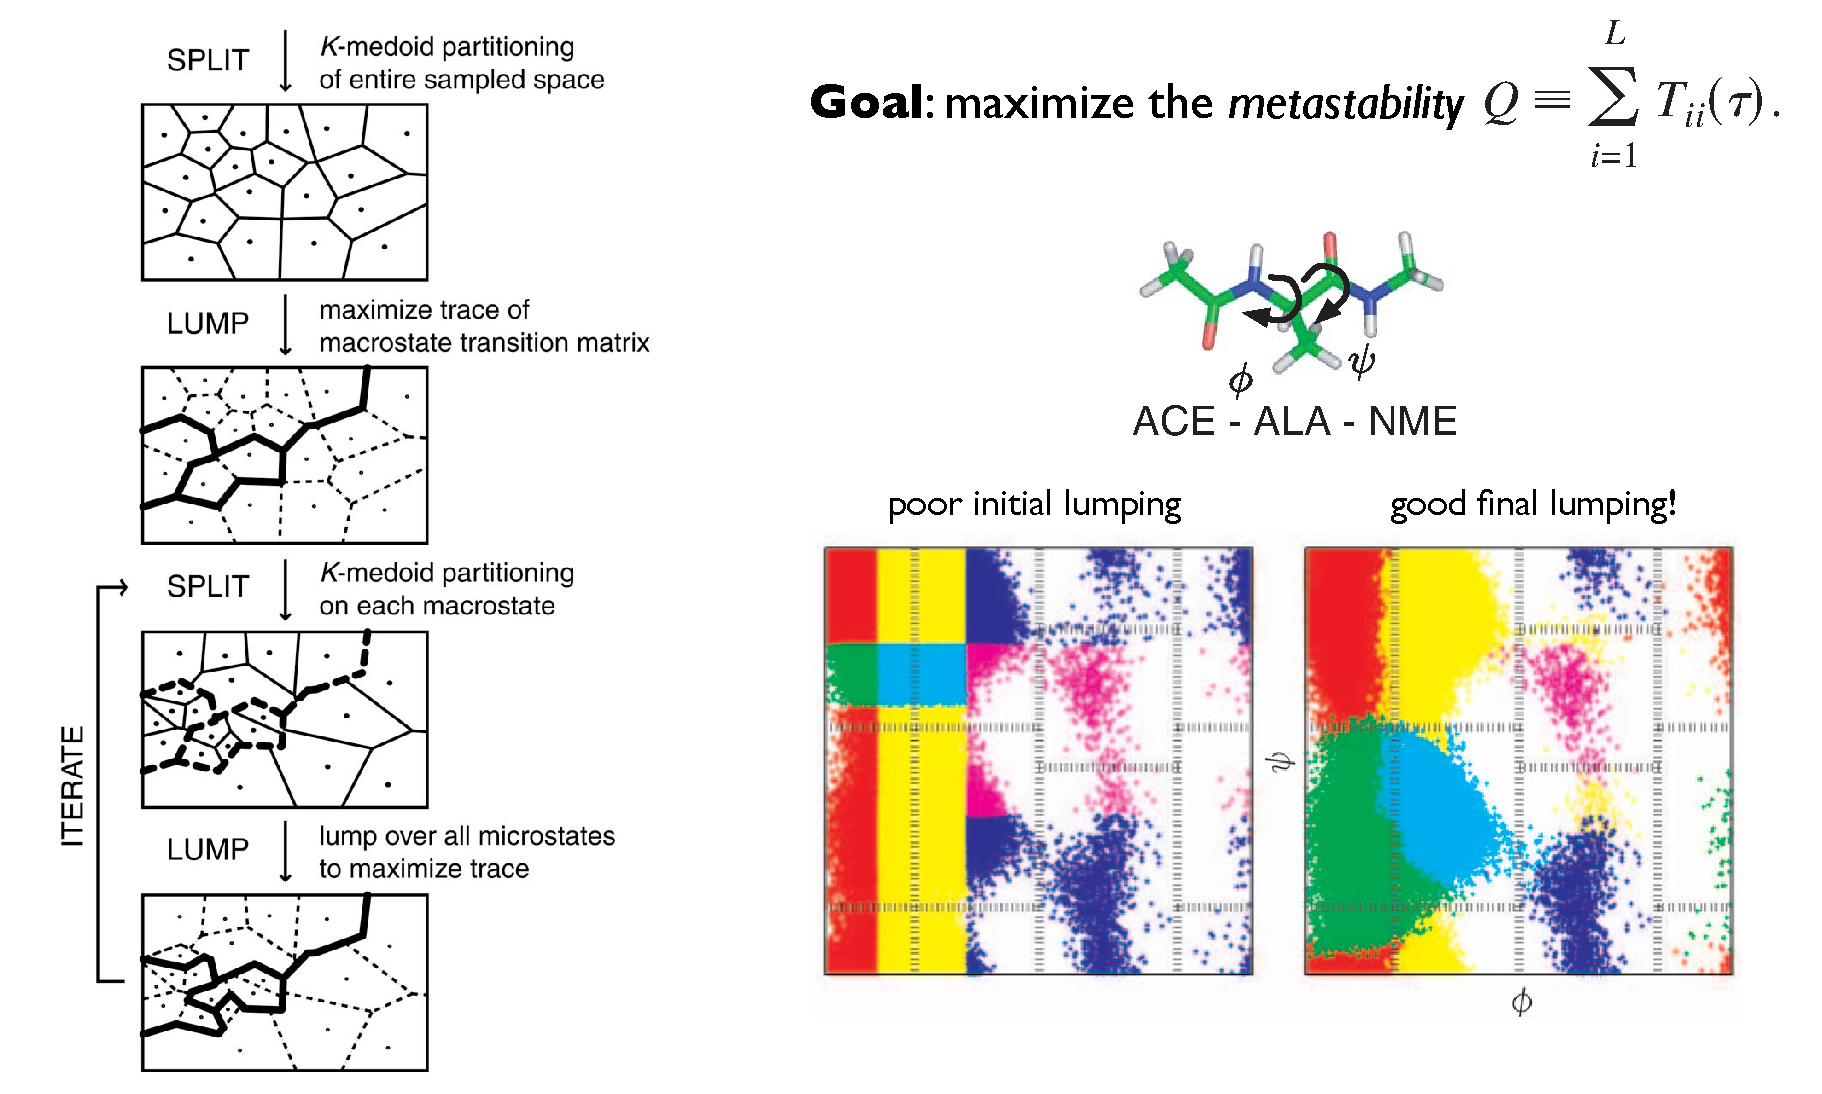
\includegraphics[width=1.0\textwidth]{metastability-lumping}
%\caption{\label{fig:your-figure}Caption goes here.}
\end{figure}

\tiny
Chodera, J. D., Singhal, N., Pande, V. S., Dill, K. A., \& Swope, W. C. (2007).The Journal of Chemical Physics, 126(15), 155101.
\normalsize

\end{frame}


%%%%%%%%%%%%%%%%%%%%%%%%%%%%%%%%%%
\begin{frame}{Automated algorithms for lumping microstates into macrostates by metastability}

Perron Cluster Cluster Analysis (PCCA) and the improved PCCA+ cluster microstates together based on the sign structure of the computed eigenvectors.  Different resolutions of course-graining cab be achieved by choosing the number of eigenvectors to include in the analysis. 

\begin{figure}
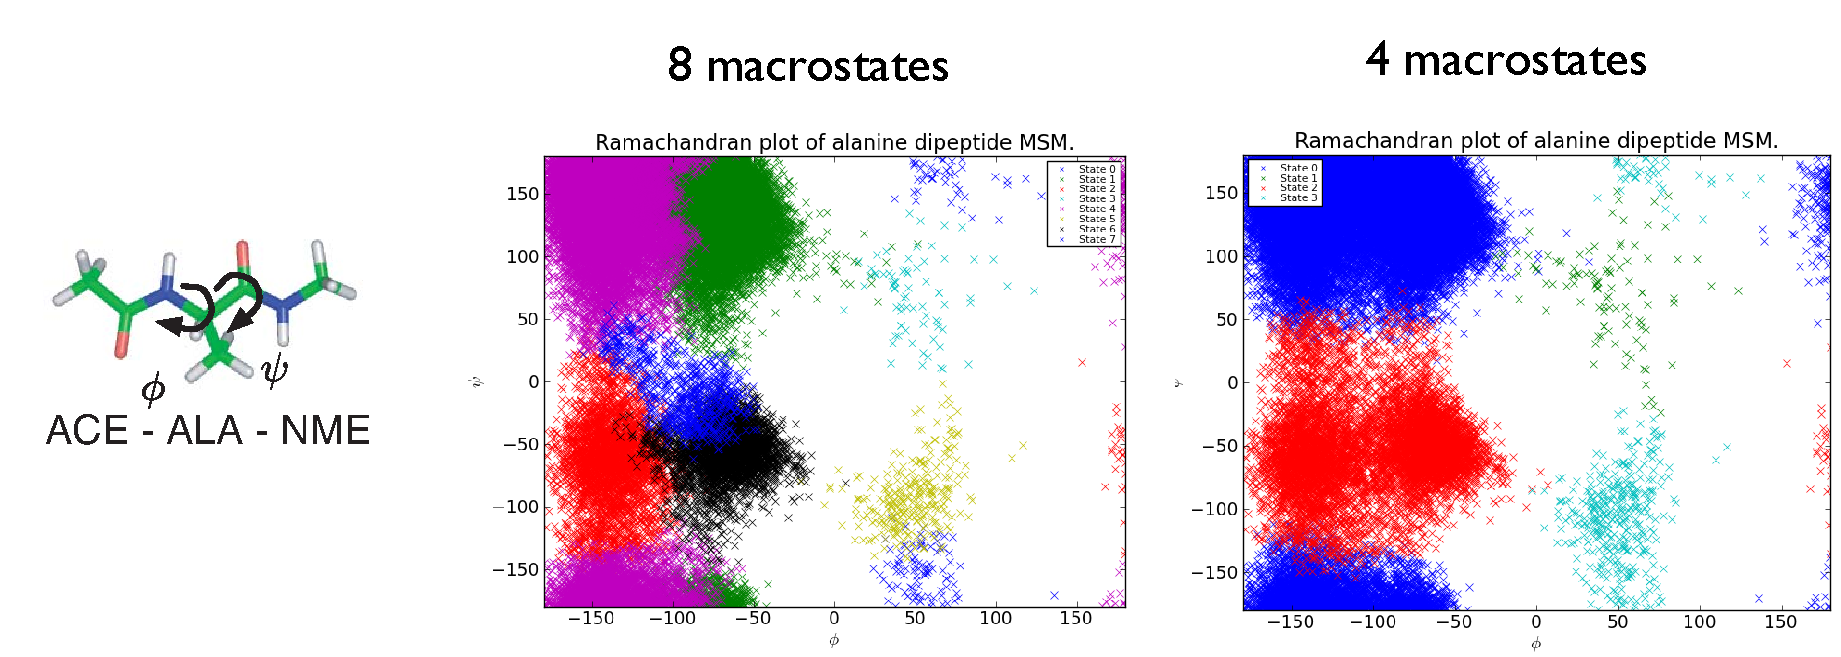
\includegraphics[width=0.7\textwidth]{PCCA-alanine}
\caption{\label{fig:PCCA-alanine}from the the MSMBuilder2 Documentation Tutorial}
\end{figure}

\tiny
P. Deuflhard, W. Huisinga, A. Fischer, C. Sch\"{u}tte, Linear Algebra Appl. 315 (2000) 39–59.
Deuflhard, P. and  Weber, M. (2005).Linear Algebra and its Applications, 398, 161–184. 
\normalsize

\end{frame}


%%%%%%%%%%%%%%%%%%%%%%%%%%%%%%%%%%
\begin{frame}{New methods for lumping look promising}



\begin{itemize}
  \item Hierarchical Nystr\"{o}m methods (Yao et al 2013)
  \item Bayesian Agglomerative Clustering Engine (BACE)  (Bowman 2012)
\end{itemize}

\tiny
Yao, Y., Cui, R. Z., Bowman, G. R., Silva, D.-A., Sun, J., and  Huang, X. (2013). Hierarchical Nystr\"{o}m methods for constructing Markov state models for conformational dynamics. The Journal of Chemical Physics, 138(17), 174106. doi:10.1063/1.4802007

Bowman, G. R. (2012). Improved coarse-graining of Markov state models via explicit consideration of statistical uncertainty. The Journal of Chemical Physics, 137(13), 134111. doi:10.1063/1.4755751
\normalsize

\end{frame}

%%%%%%%%%%%%%%%%%%%%%%%%%%%%%%%%%%
\begin{frame}{...but the best partition is \textit{not} necessarily metastable}


\begin{wrapfigure}{l}{0.5\textwidth}
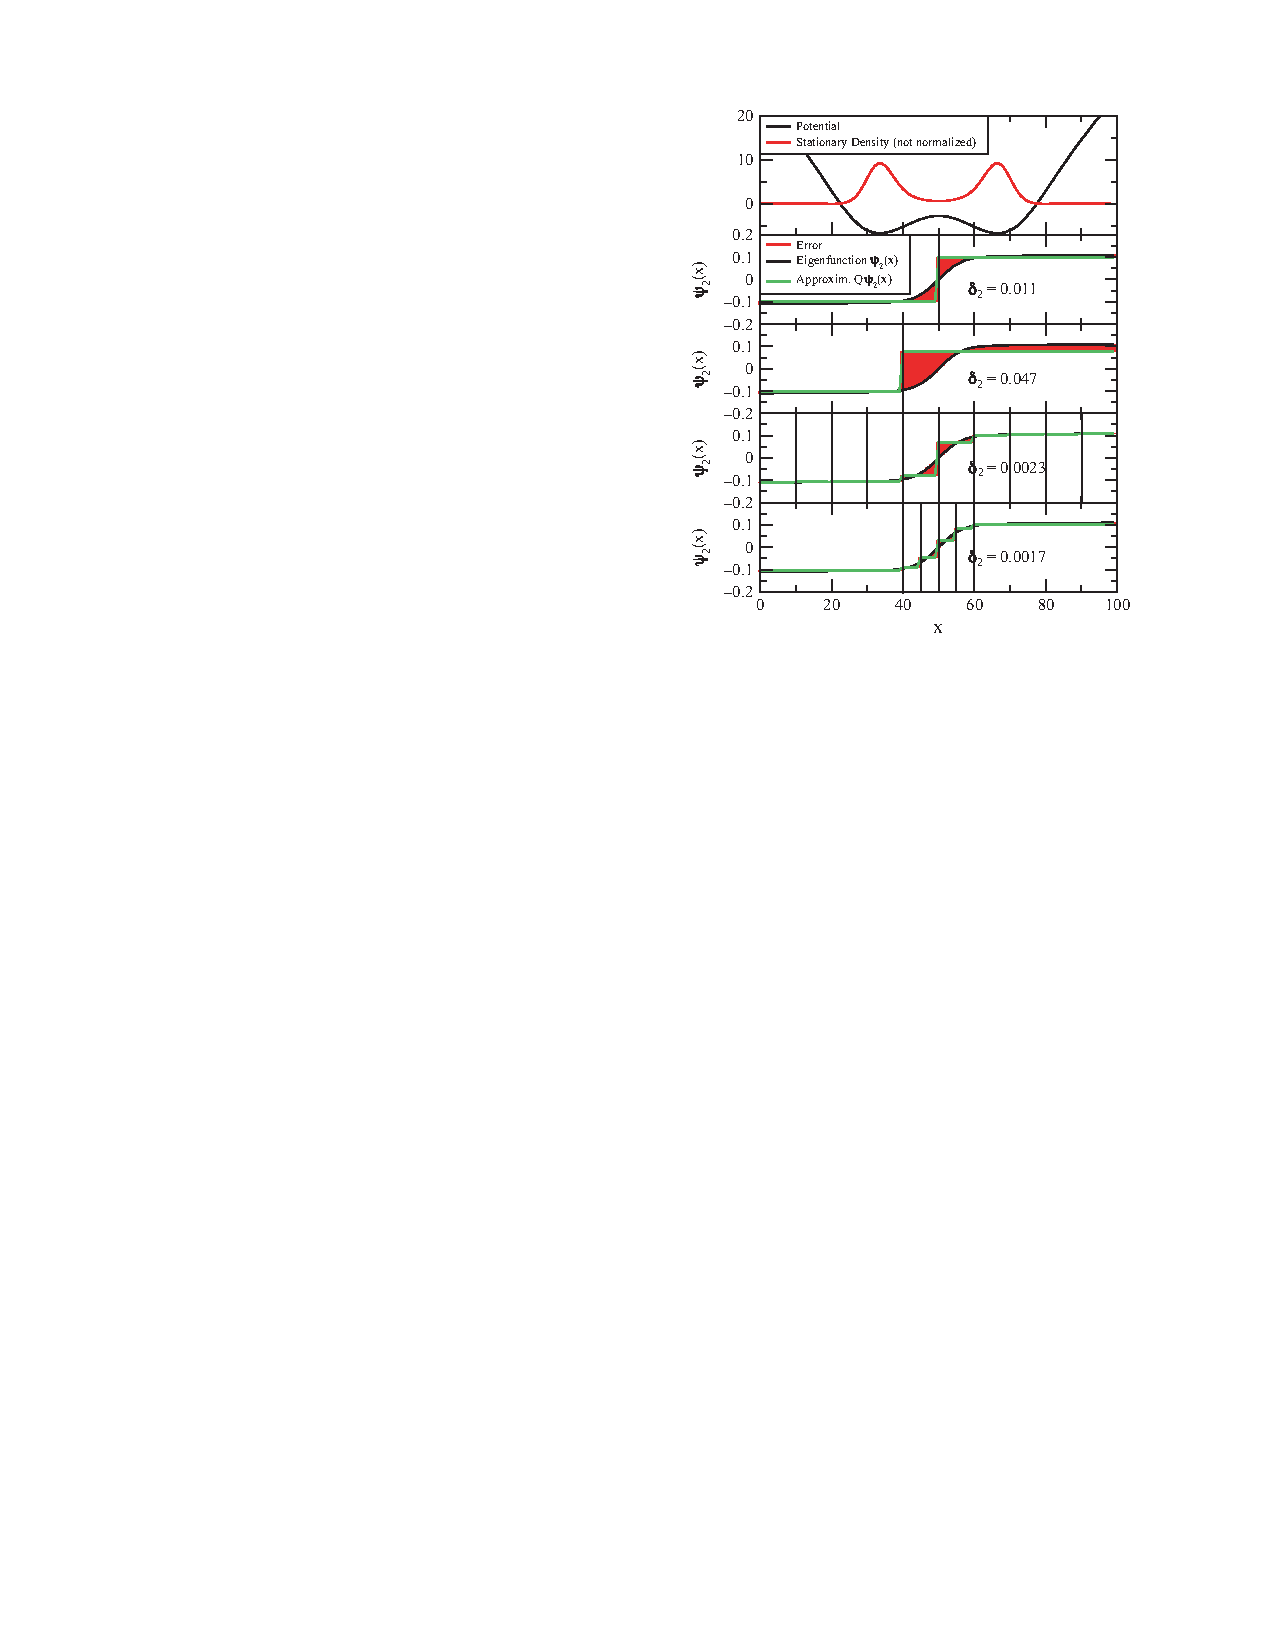
\includegraphics[width=0.48\textwidth]{discretization-error}
%\caption{\label{fig:discretization-error}}
\end{wrapfigure}

\small
The catch: Keeping many fine-grained states near transition barriers can arbitrarily improve \textit{discretization} error, but at the expense of finite sampling error (i.e. sample enough transitions to make good estimates)   
\normalsize

\tiny
Prinz, J.-H., Wu, H., Sarich, M., Keller, B., Senne, M., Held, M., et al. (2011). Markov models of molecular kinetics: generation and validation. The Journal of Chemical Physics, 134(17), 174105. doi:10.1063/1.3565032
\normalsize

\end{frame}


%%%%%%%%%%%%%%%%%%%%%%%%%%%%%%%%%%
\begin{frame}{Playing it safe: Define states and lump using predefined reaction coordinates}

For this HIV-1 protease system, the important degrees of freedom are already known
\begin{figure}
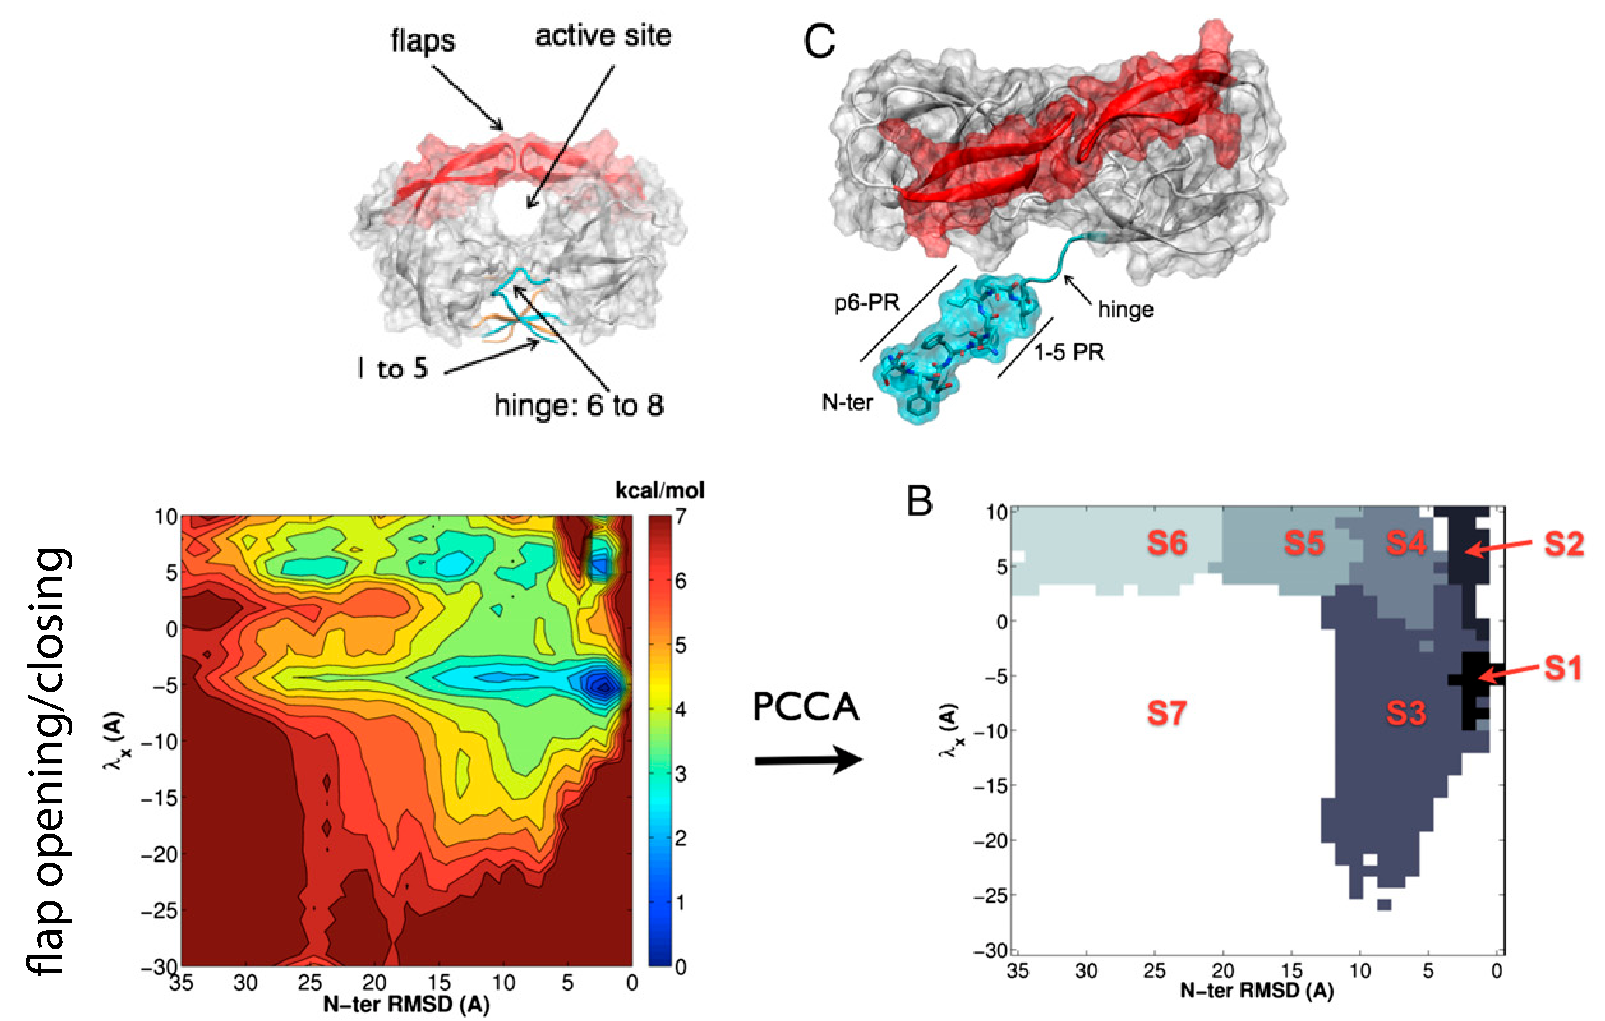
\includegraphics[width=0.7\textwidth]{HIV-flap}
%\caption{\label{fig:b}b}
\end{figure}


\tiny
Sadiq, S. K., Noé, F., and De Fabritiis, G. (2012). Kinetic characterization of the critical step in HIV-1 protease maturation. PNAS, 109(50), 20449–20454. doi:10.1073/pnas.1210983109
\normalsize

\end{frame}


%%%%%%%%%%%%%%%%%%%%%%%%%%%%%%%%%%
\begin{frame}{Transition Path Theory}

\textbf{Transition Path Theory} (TPT) is a method to compute steady-state (equilibrium) net folding fluxes.  Like master equation kinetics, TPT fluxes for MSMs can be computed entirely from the transition matrix $\mathbf{T}^{(\tau)}$

\begin{figure}
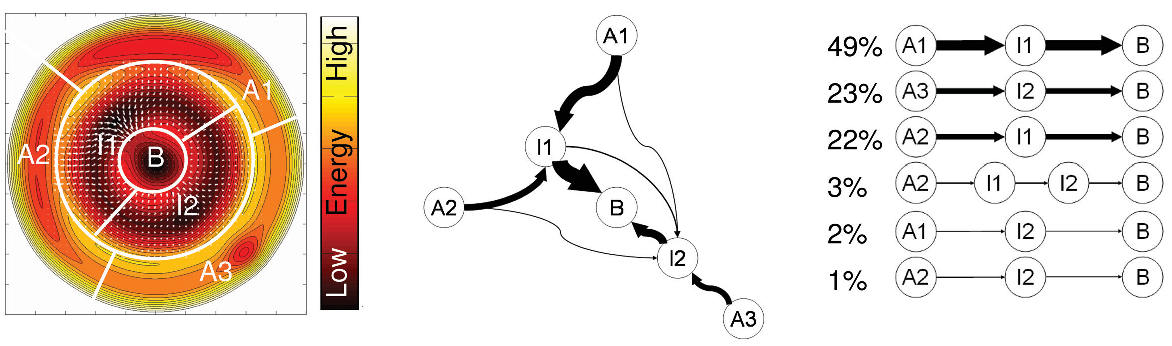
\includegraphics[width=0.85\textwidth]{TPT-Noe}
%\caption{\label{fig:b}b}
\end{figure}


\tiny
No\'{e}, F., Sch\"{u}tte, C., Vanden-Eijnden, E., Reich, L., and  Weikl, T. R. (2009). Constructing the equilibrium ensemble of folding pathways from short off-equilibrium simulations. PNAS, 106(45), 19011–19016. doi:10.1073/pnas.0905466106

Metzner, P., Sch\"{u}tte, C., and Vanden-Eijnden, E. (2009). Transition Path Theory for Markov Jump Processes. Multiscale Modeling \& Simulation, 7(3), 1192. doi:10.1137/070699500
\normalsize

\end{frame}


%%%%%%%%%%%%%%%%%%%%%%%%%%%%%%%%%%
\begin{frame}{Transition Path Theory}

Heterogeneous folding pathways in PinWW domain
\begin{figure}
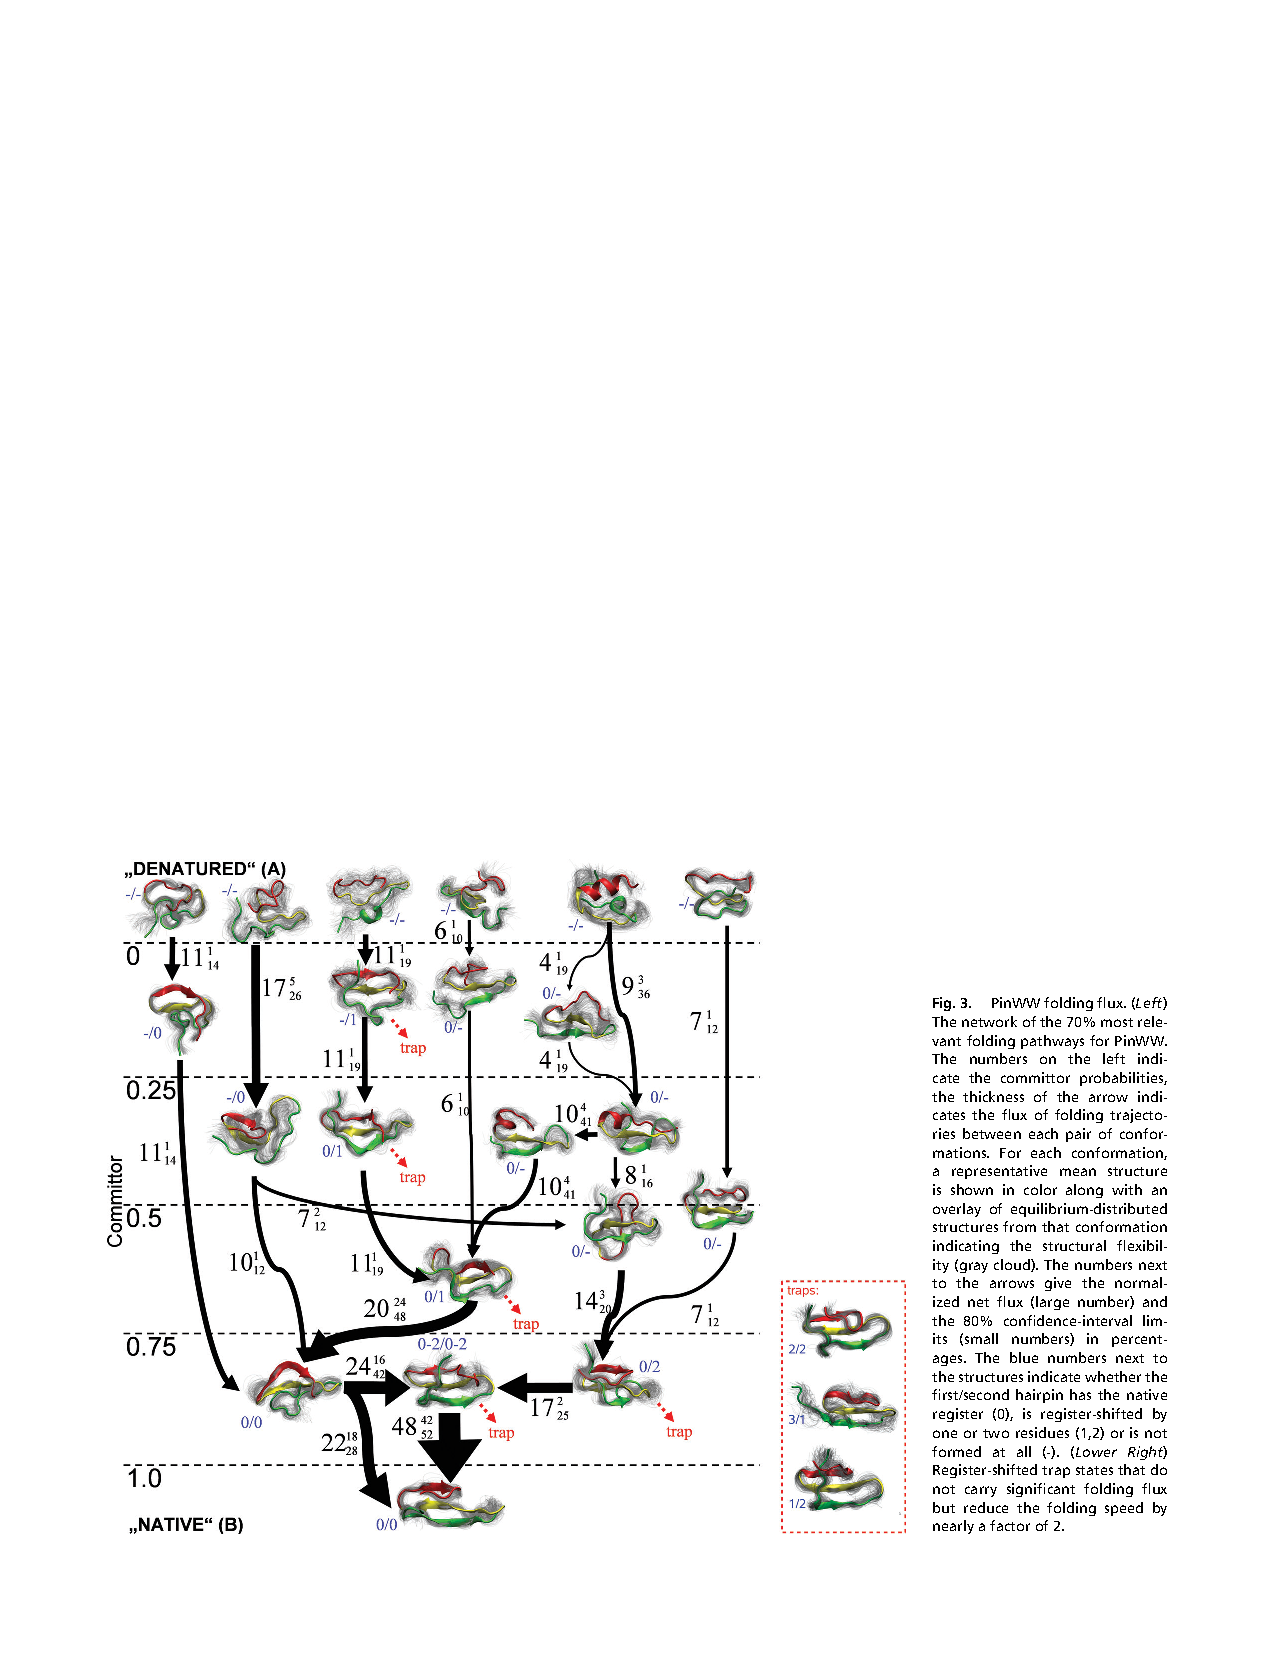
\includegraphics[width=0.85\textwidth]{TPT-wwdomain}
%\caption{\label{fig:b}b}
\end{figure}

\tiny
No\'{e}, F., Sch\"{u}tte, C., Vanden-Eijnden, E., Reich, L., and  Weikl, T. R. (2009). Constructing the equilibrium ensemble of folding pathways from short off-equilibrium simulations. PNAS, 106(45), 19011–19016. doi:10.1073/pnas.0905466106
\normalsize

\end{frame}




%%%%%%%%%%%%%%%%%%%%%%%%%%%%%%%%%%
\begin{frame}{Transition Path Theory}

Two dominant pathways in NTL9(1-39) folding differ in hairpin registration

\begin{figure}
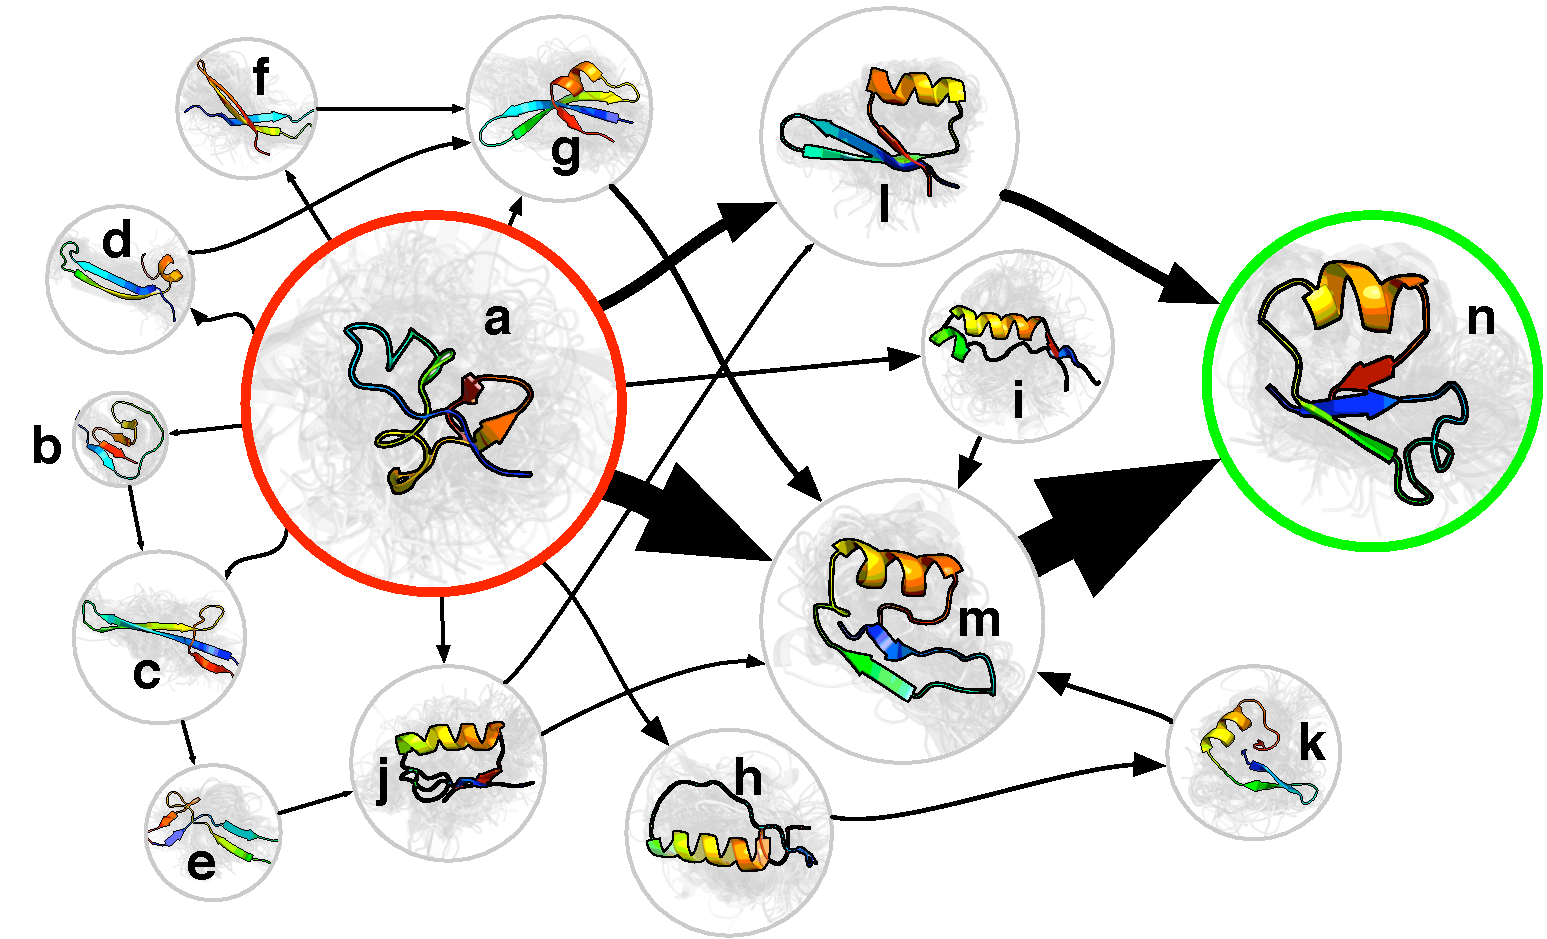
\includegraphics[width=0.85\textwidth]{TPT-ntl9}
%\caption{\label{fig:b}b}
\end{figure}


\tiny
Voelz, V. A., Bowman, G. R., Beauchamp, K., \& Pande, V. S. (2010). Molecular simulation of ab initio protein folding for a millisecond folder NTL9(1-39). JACS, 132(5), 1526–1528. doi:10.1021/ja9090353
\normalsize

\end{frame}


%%%%%%%%%%%%%%%%%
\begin{frame}{Conclusions}

\texttt{MSMBuilder} is a useful tool for

\begin{itemize}
  \item discovering the relevant metastable states
  \item validating the assumption that dynamics is ``Markovian''
  \item mstimating the master equation kinetics 
  \item making human sense of such huge networks
\end{itemize}

You should try it today!  \texttt{https://github.com/SimTk/msmbuilder.git}

\end{frame}





\end{document}
